\clearpage

\subsection{Scale factors}

In~\ref{sec:object-selection-electrons} and~\ref{sec:muon-selection} we have studied the selection we apply to electrons and muons respectively. We have therewith made a choice about identification working point. We have used simulation exclusively to draw conclusions about the identification efficiency of the leptons. If we rely on \gls{mc} simulation,  that will produce large systematic errors due to imperfections in modeling both the data and the detector response. We therefore wish to measure the identification efficiency in data, in order to correct the simulation's potentially false efficiency rate. \emph{Efficiency} is defined as how probable it is to reconstruct or identify a lepton. For a lepton $\ell$ the identification efficiency is defined as:

\begin{equation}
\varepsilon_{\ell}^{\mathrm{ID}} = \frac{N_{\ell}(\mathrm{ID})}{N_{\ell}(\mathrm{produced})}
\end{equation}

In \gls{mc} simulation, the number of leptons produced is the same as the number of leptons generated. In data, one must measure it using a data-driven method. Once the efficiencies have been measured both in simulation and in data, a correction factor named \gls{sf} can be applied to the simulation in order to correct for any discrepancies that might arise. The scale factors are defined as the ratio between the efficiency in data to the efficiency in simulation:

\begin{equation}
\mathrm{SF}_{\ell}^{\mathrm{ID}}=\frac{\varepsilon_{\ell}^{\mathrm{ID,Data}}}{\varepsilon_{\ell}^{\mathrm{ID,MC}}},
\end{equation}

dropping the superscript ID we get:

\begin{equation}
\mathrm{SF}_{\ell}=\frac{\varepsilon_{\ell}^{\mathrm{Data}}}{\varepsilon_{\ell}^{\mathrm{MC}}}.
\end{equation}

Once the relevant \gls{sf} have been determined, they are applied for every lepton passing the object selection in the event. The scale factors for loose-ID electrons in our \pt range have been measured centrally by the relevant working group and are applied to the selected electrons. As was determined in~\ref{sec:muon-selection}, our analysis signal muon's lower \pt threshold is $2\GeV$ which is low. Scale factors for medium ID leptons with $\pt\geq 2\GeV$ were computed centrally by the Muon \gls{pog}. The scale factors, however, while matching our muons' \pt range and identification working point, were computed by requiring $\DR > 0.5$  between the muons~\cite{muon-id-sf-2016,muon-id-sf-2016-pres}. As we have seen in~\ref{sec:lepton-dr}, one of are drivers of the sensitivity is the region of $\DR < 0.5$. We would therefore like to validate the scale factors in that region. We would like to show that the efficiencies have no $\DR$ dependence, and in order to do so, we calculate the efficiencies in different $\DR$ regions.

In order to measure such efficiency in data, one must identify desired leptons with low and easily reducible fakes. A widely used method to perform such a data-driven task is the Tag \& Probe method. In the Tag \& Probe method we examine a mass resonance such as \PZ, \JPsi or \PGU to select particles of the desired type, and probe the efficiency of a particular selection criterion on those particles. The mass resonance will then decay into two same-flavor opposite charged pair of leptons and will form a peak on top of a background. Since we are interested in measuring the efficiency of low \pt muons, we choose to look at dimuon events around the \JPsi mass window. In a dimuon event, we describe one muon as a `tag' and the other as a `probe'. The tag muon is selected with a very tight selection which results in very high certainty that the object corresponds to a real muon produced. The probe is given a loose selection, but since it is constrained to be consistent with a product of a \JPsi, it is almost certain that originate from a real muon too. Since the shape of the \JPsi is a peak over a background, the background is easily removed by fits. The probe is then subjected to cuts or constraints which are used to measure a particular efficiency. As stated, in this study we want to show that the efficiency to identify a muon with medium ID working point from a track has no $\DR$ depandance. Therefore, the efficiency we are looking for is defined as:

\begin{equation}
\varepsilon_{\mu}^{\mathrm{ID}} = \frac{N_{\mu}^\mathrm{ID}}{N_{t}}.
\end{equation}

The probe we are using in the denominator is a track passing a loose selection, while the probe track in the denominator is required to match a medium ID working point muon. The number of objects passing a selection is determined by a fit to data and \gls{mc}, to measure the corresponding efficiencies in data and \gls{mc}.

This study is done for year 2016. For the \gls{mc}, we are using the 2016 samples listed in~\ref{sec:sm-mc}. For data, we are  using a single electron trigger, in order for the tagged muon to be independent from the triggered object. he data set is measured to correspond to 36.02\fbinv using the BRIL Work Suite~\cite{bril}. The following trigger paths are used:

\begin{itemize}
\item \texttt{HLT\_Ele27\_WPTight\_Gsf\_v*},
\item \texttt{HLT\_Ele27\_eta2p1\_WPLoose\_Gsf\_v*},
\item \texttt{HLT\_Ele32\_WPTight\_Gsf\_v*},
\item \texttt{HLT\_Ele35\_WPTight\_Gsf\_v*}.
\end{itemize}

We then select an offline loose ID electron with $\pt>27\GeV$ offline. The requirement to select a tag \& probe pair are defined in table~\ref{tab:tag-probe-def}.

\begin{table}[!htb]
	\centering
	\label{tab:tag-probe-def}
		\caption{Selection criteria for Tags and Probes}
		%\vspace{1mm}
			\begin{tabular}{l|l} \hline
			Tag & Probe \\ \hline
			medium ID muon & isolated track\\
			$\pt \geq 5\GeV$ & $2\leq\pt\leq 20\GeV$  ($ \pt\geq 3 \GeV $ for barrel) \\
			$\abs{\eta}<2.4$ & opposite-sign in invariant mass window $[2.5,3.5]\GeV$ \\ \hline
			\end{tabular}
\end{table}

A fit is then performed in an invariant mass window around the \JPsi window of $[2.5,3.5]\GeV$. The signal fit is using a crystal ball function and the continuum is fit with a 6th order polynomial. The fit is repeated twice, where the denominator is done with probe tracks, and the numerator is using medium ID muons that have been matched to said tracks. The \DR~range has been split into 3, and $\abs{\eta}$ of the muons has been split into barrel ($\abs{\eta}<1.2$) and endcaps ($1.2<\abs{\eta}<2.4$). Simulation fits are shown in~\ref{fig:tb-barrel-simulation} for barrel, and~\ref{fig:tb-endcaps-simulation} for endcaps. Data fits are shown in~\ref{fig:tb-barrel-data} for barrel, and~\ref{fig:tb-endcaps-data} for endcaps.

\begin{figure}[!htbp]
\centering
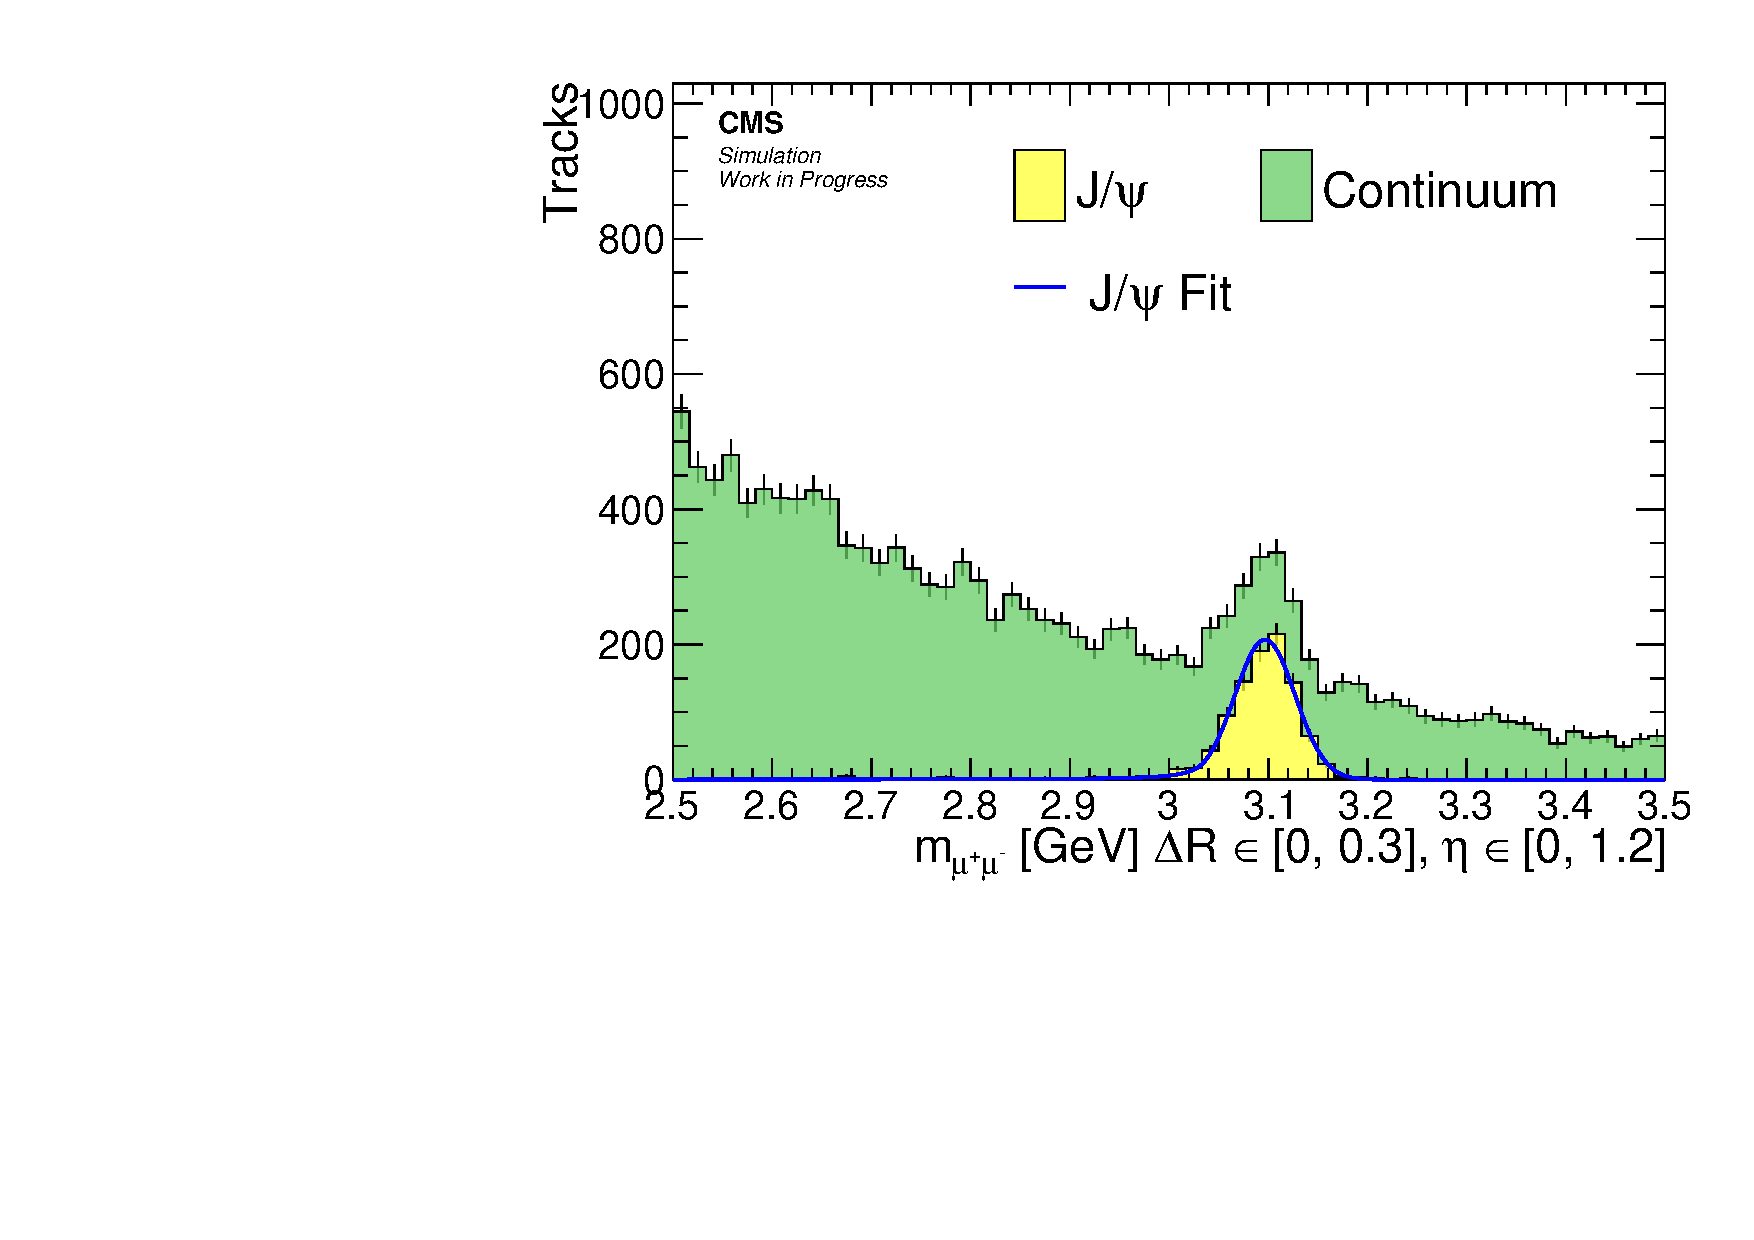
\includegraphics[width=0.32\linewidth]{plots/jpsi_muons_fit_bg_delta_r_single_electron/none_invMass_0_0.3_0_1.2.pdf} \,
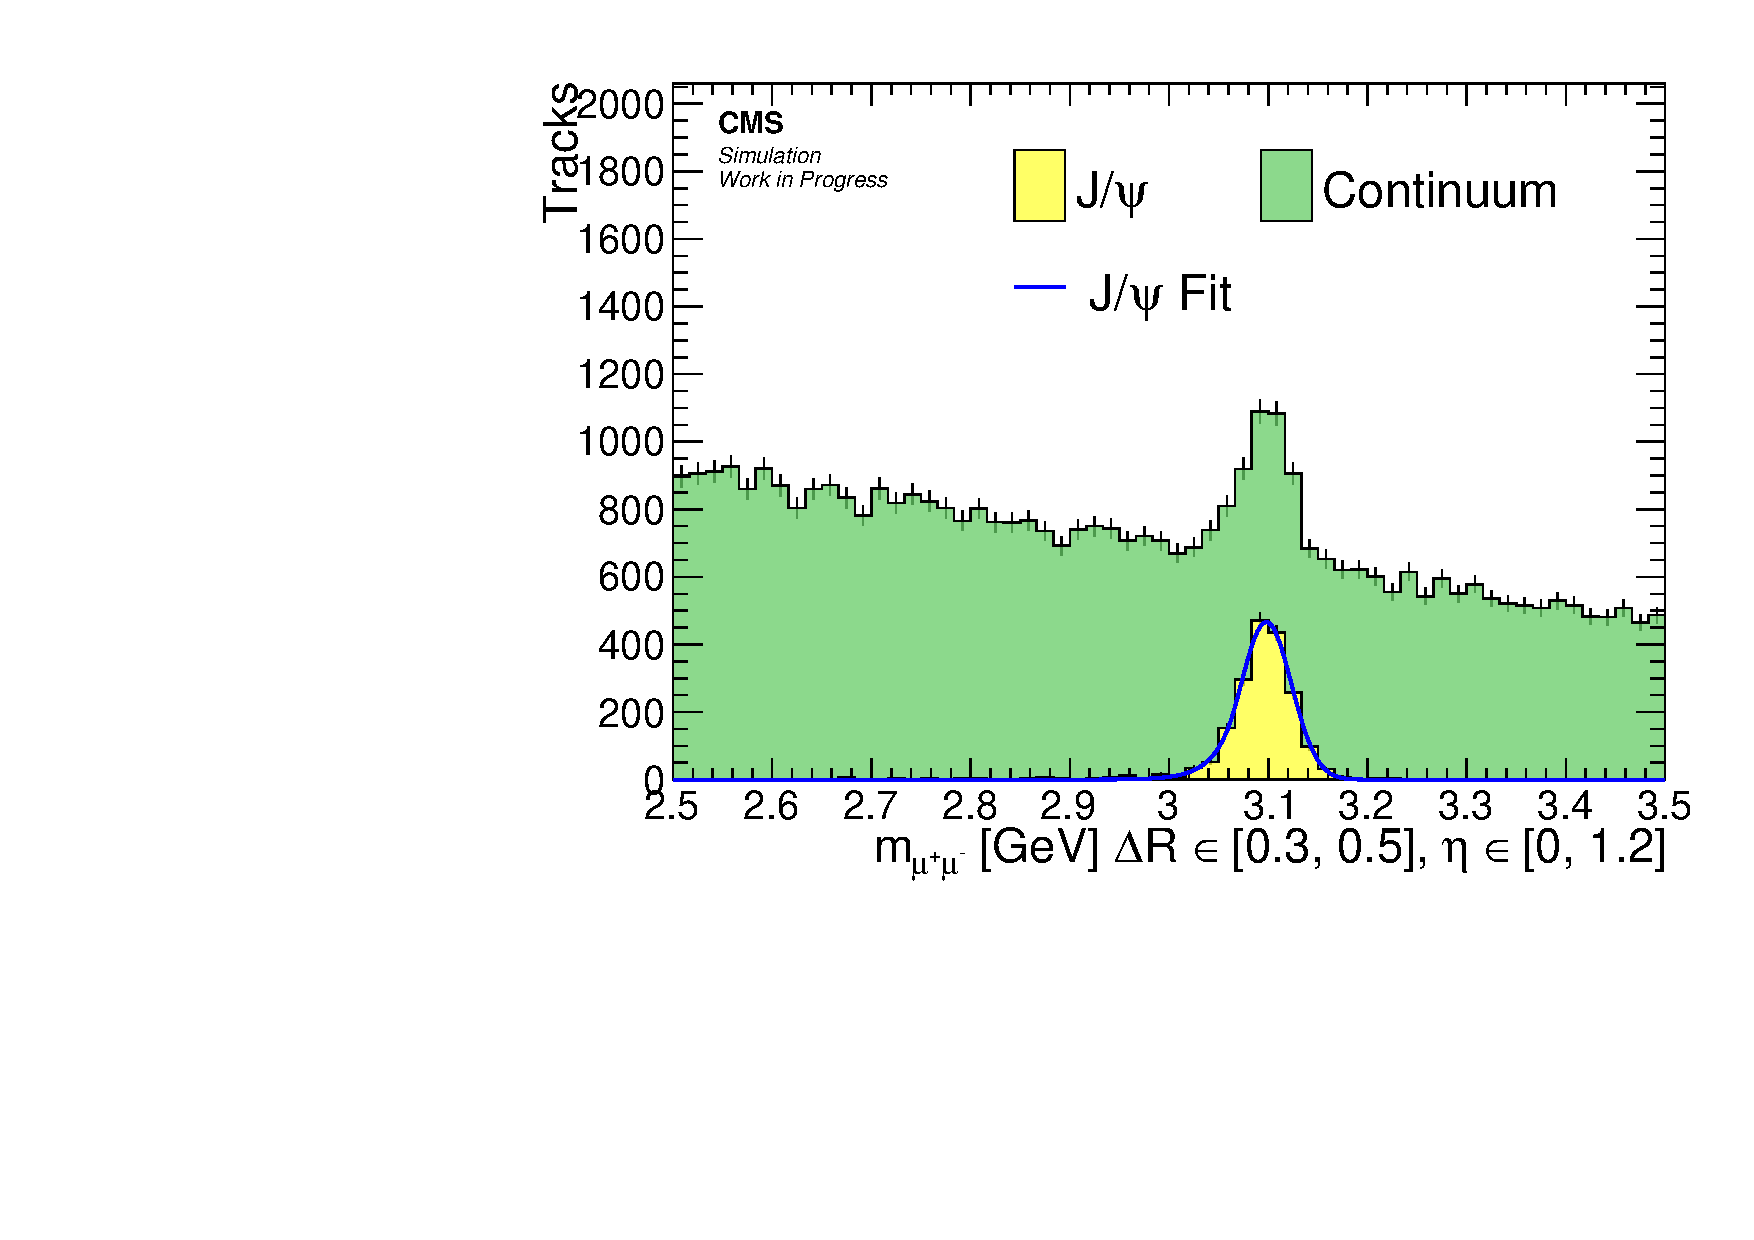
\includegraphics[width=0.32\linewidth]{plots/jpsi_muons_fit_bg_delta_r_single_electron/none_invMass_0.3_0.5_0_1.2.pdf}  \,
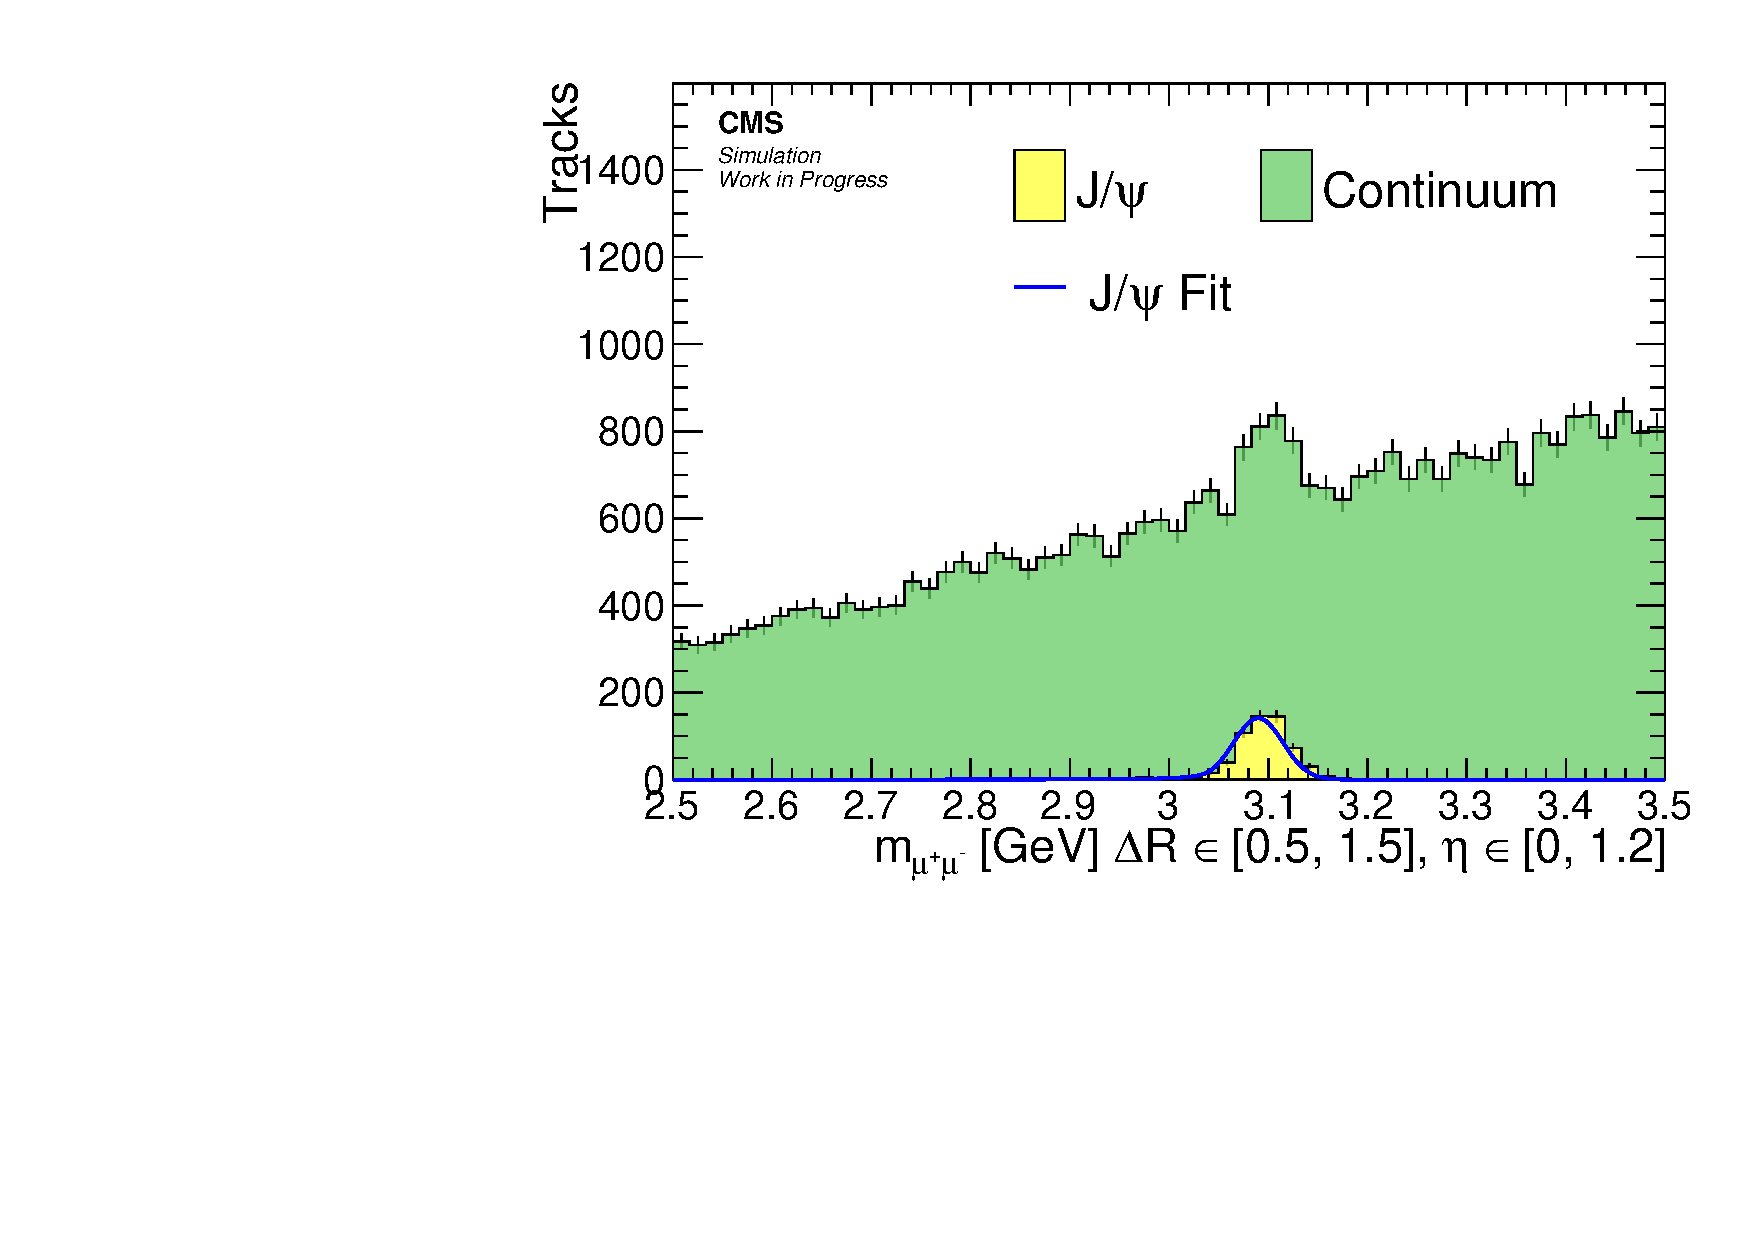
\includegraphics[width=0.32\linewidth]{plots/jpsi_muons_fit_bg_delta_r_single_electron/none_invMass_0.5_1.5_0_1.2.pdf} \\
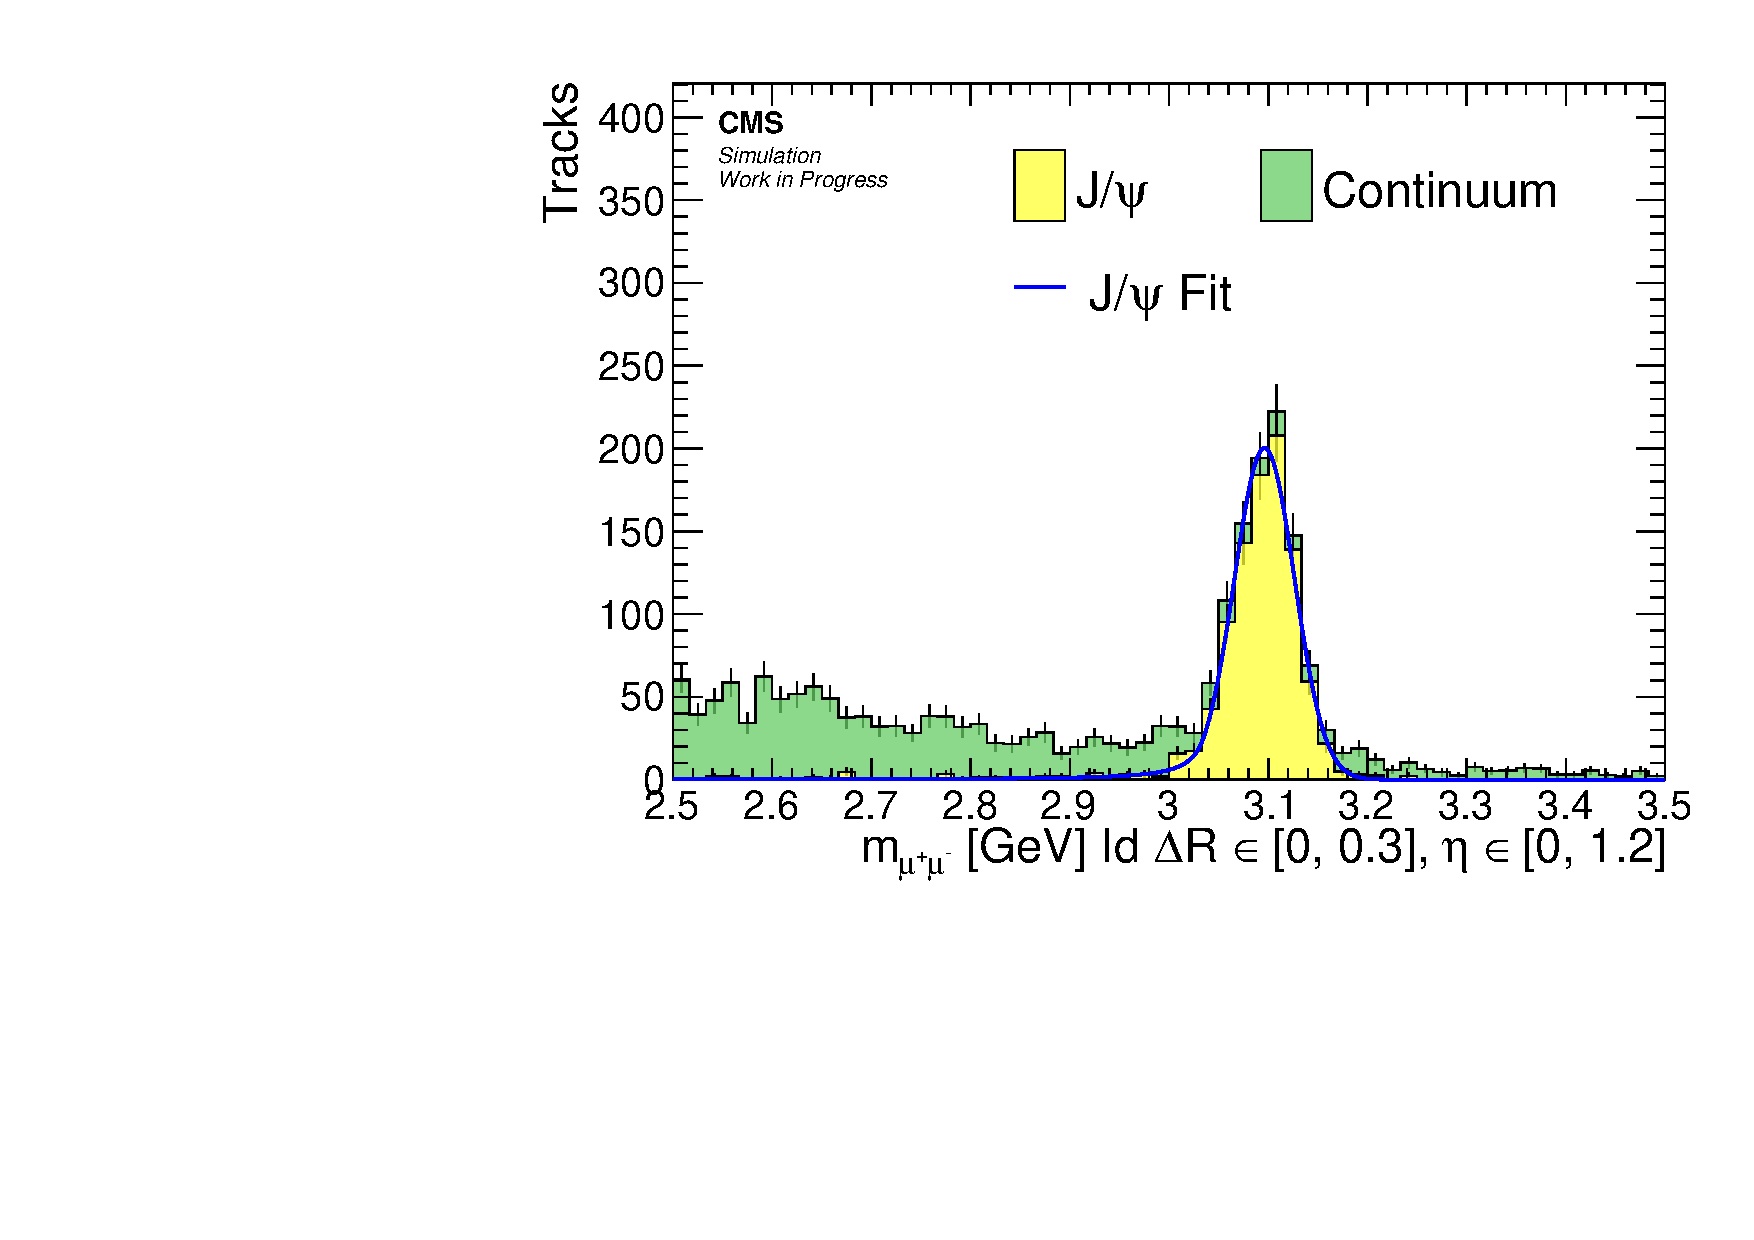
\includegraphics[width=0.32\linewidth]{plots/jpsi_muons_fit_bg_delta_r_single_electron/none_id_invMass_0_0.3_0_1.2.pdf} \,
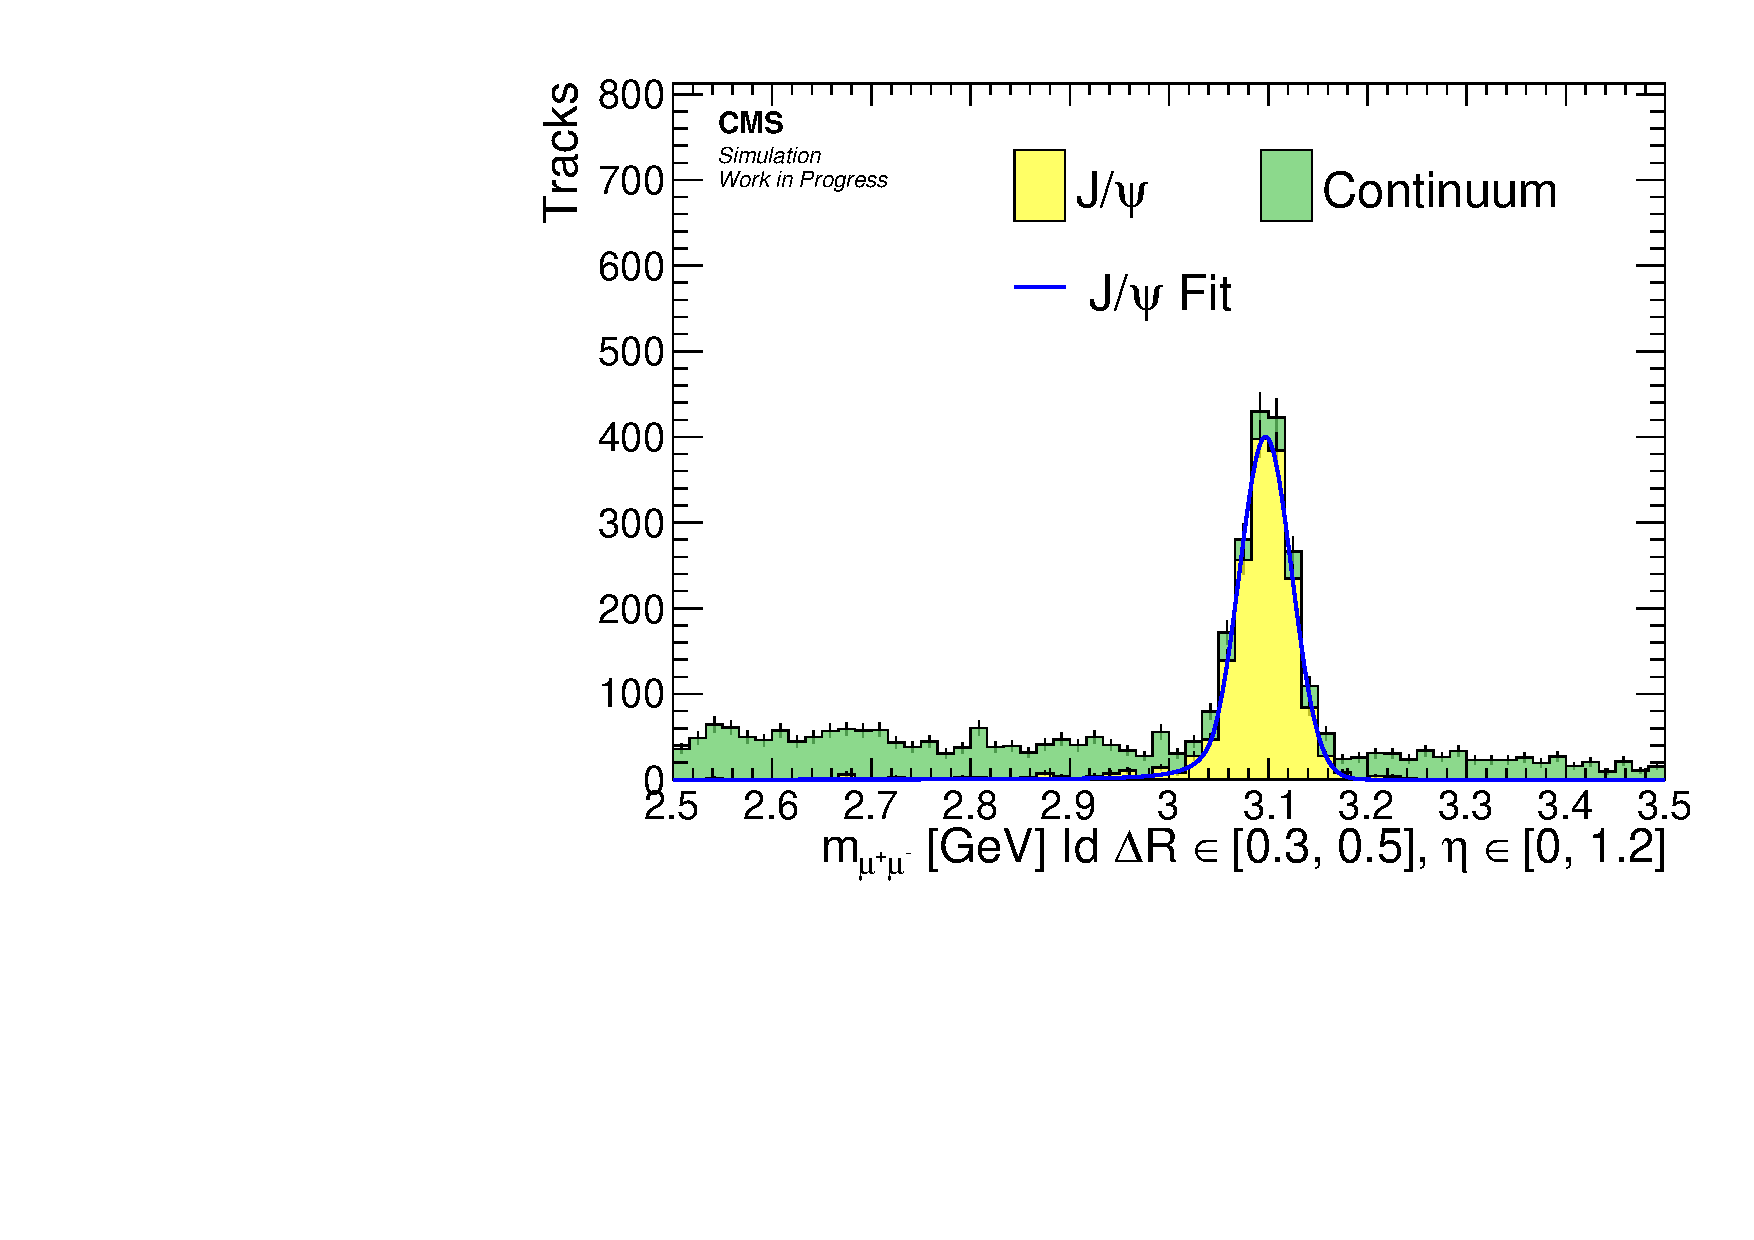
\includegraphics[width=0.32\linewidth]{plots/jpsi_muons_fit_bg_delta_r_single_electron/none_id_invMass_0.3_0.5_0_1.2.pdf}  \,
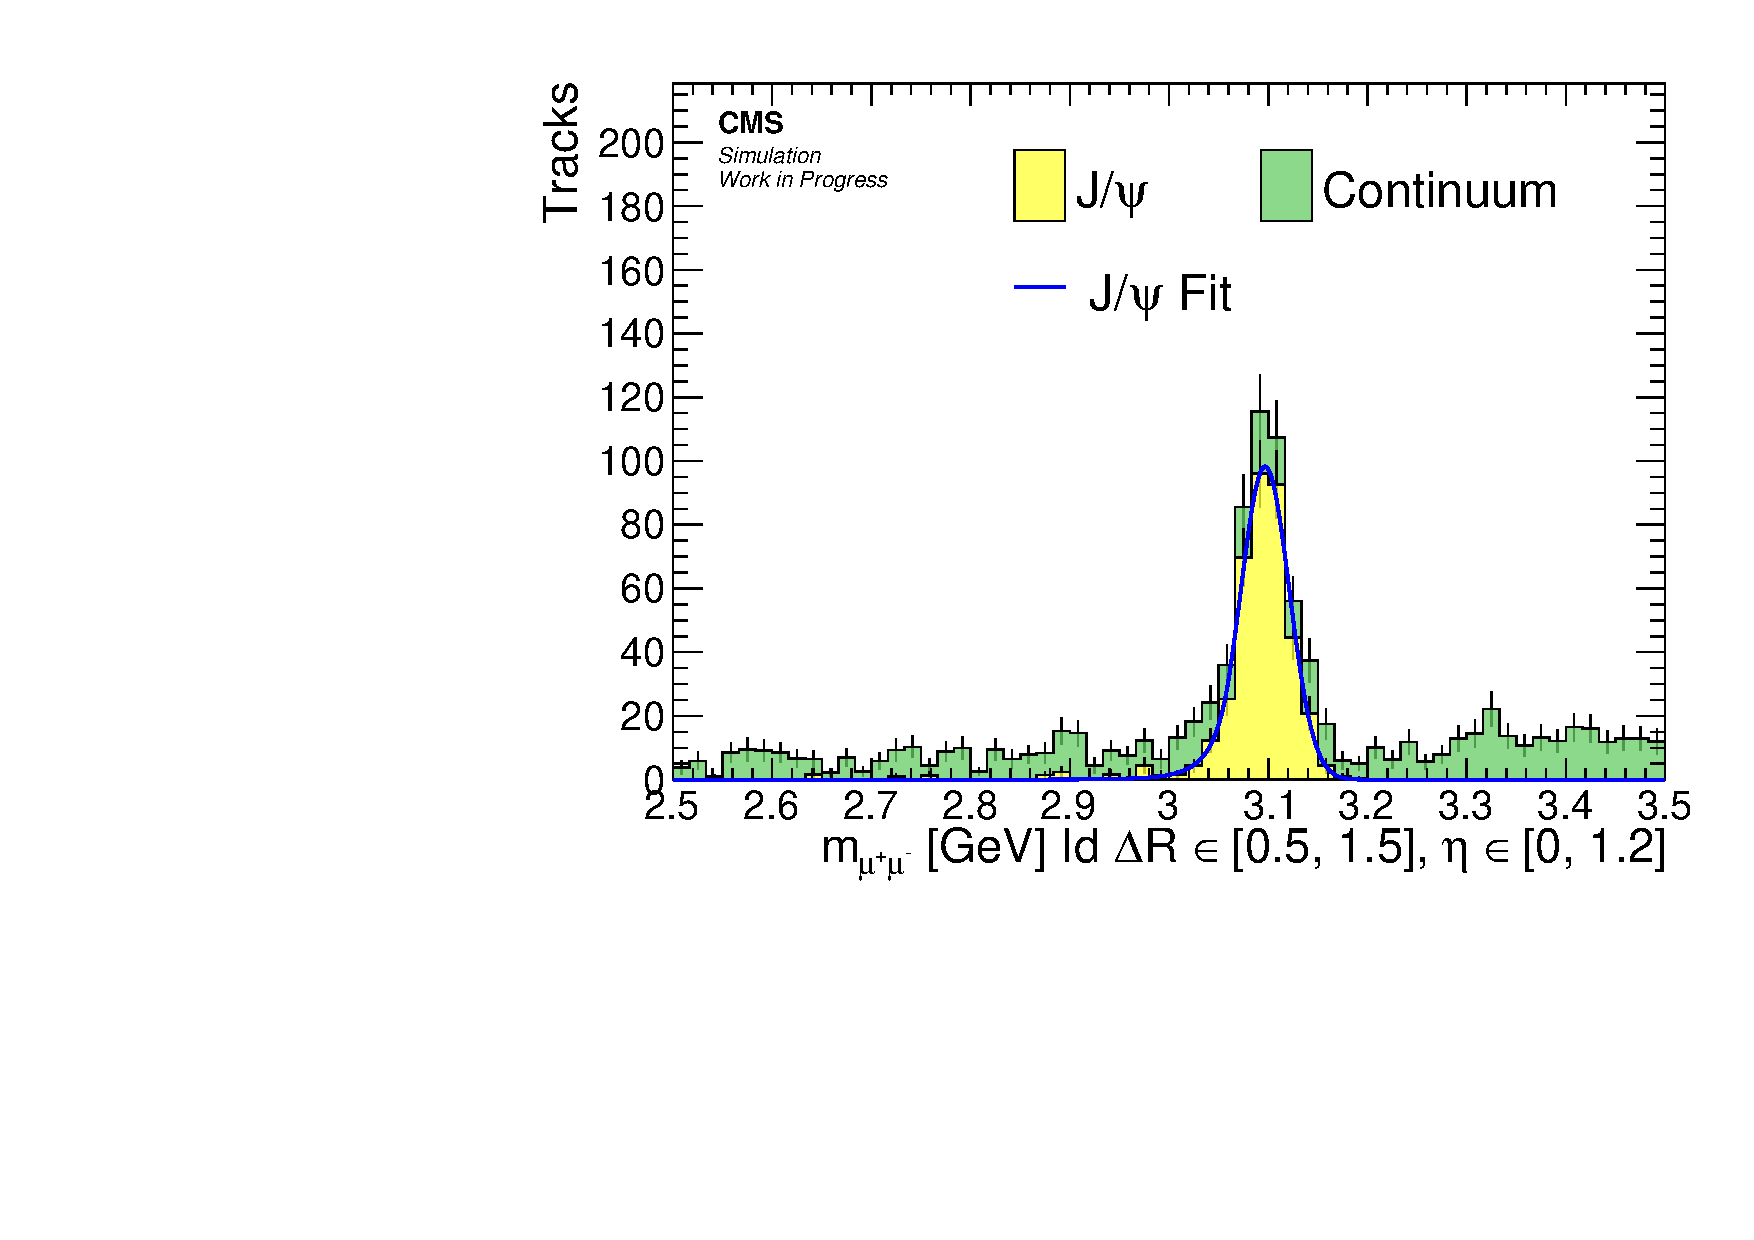
\includegraphics[width=0.32\linewidth]{plots/jpsi_muons_fit_bg_delta_r_single_electron/none_id_invMass_0.5_1.5_0_1.2.pdf} \\
\caption[Simluation barrel muons fits]{Simluation barrel muons fits for denominator (top) and numerator (bottom) for $0<\DR<0.3$  (left), $0.3<\DR<0.5$ (center), $0.5<\DR<1.5$ (right)}
\label{fig:tb-barrel-simulation}
\end{figure}

\begin{figure}[!htbp]
\centering
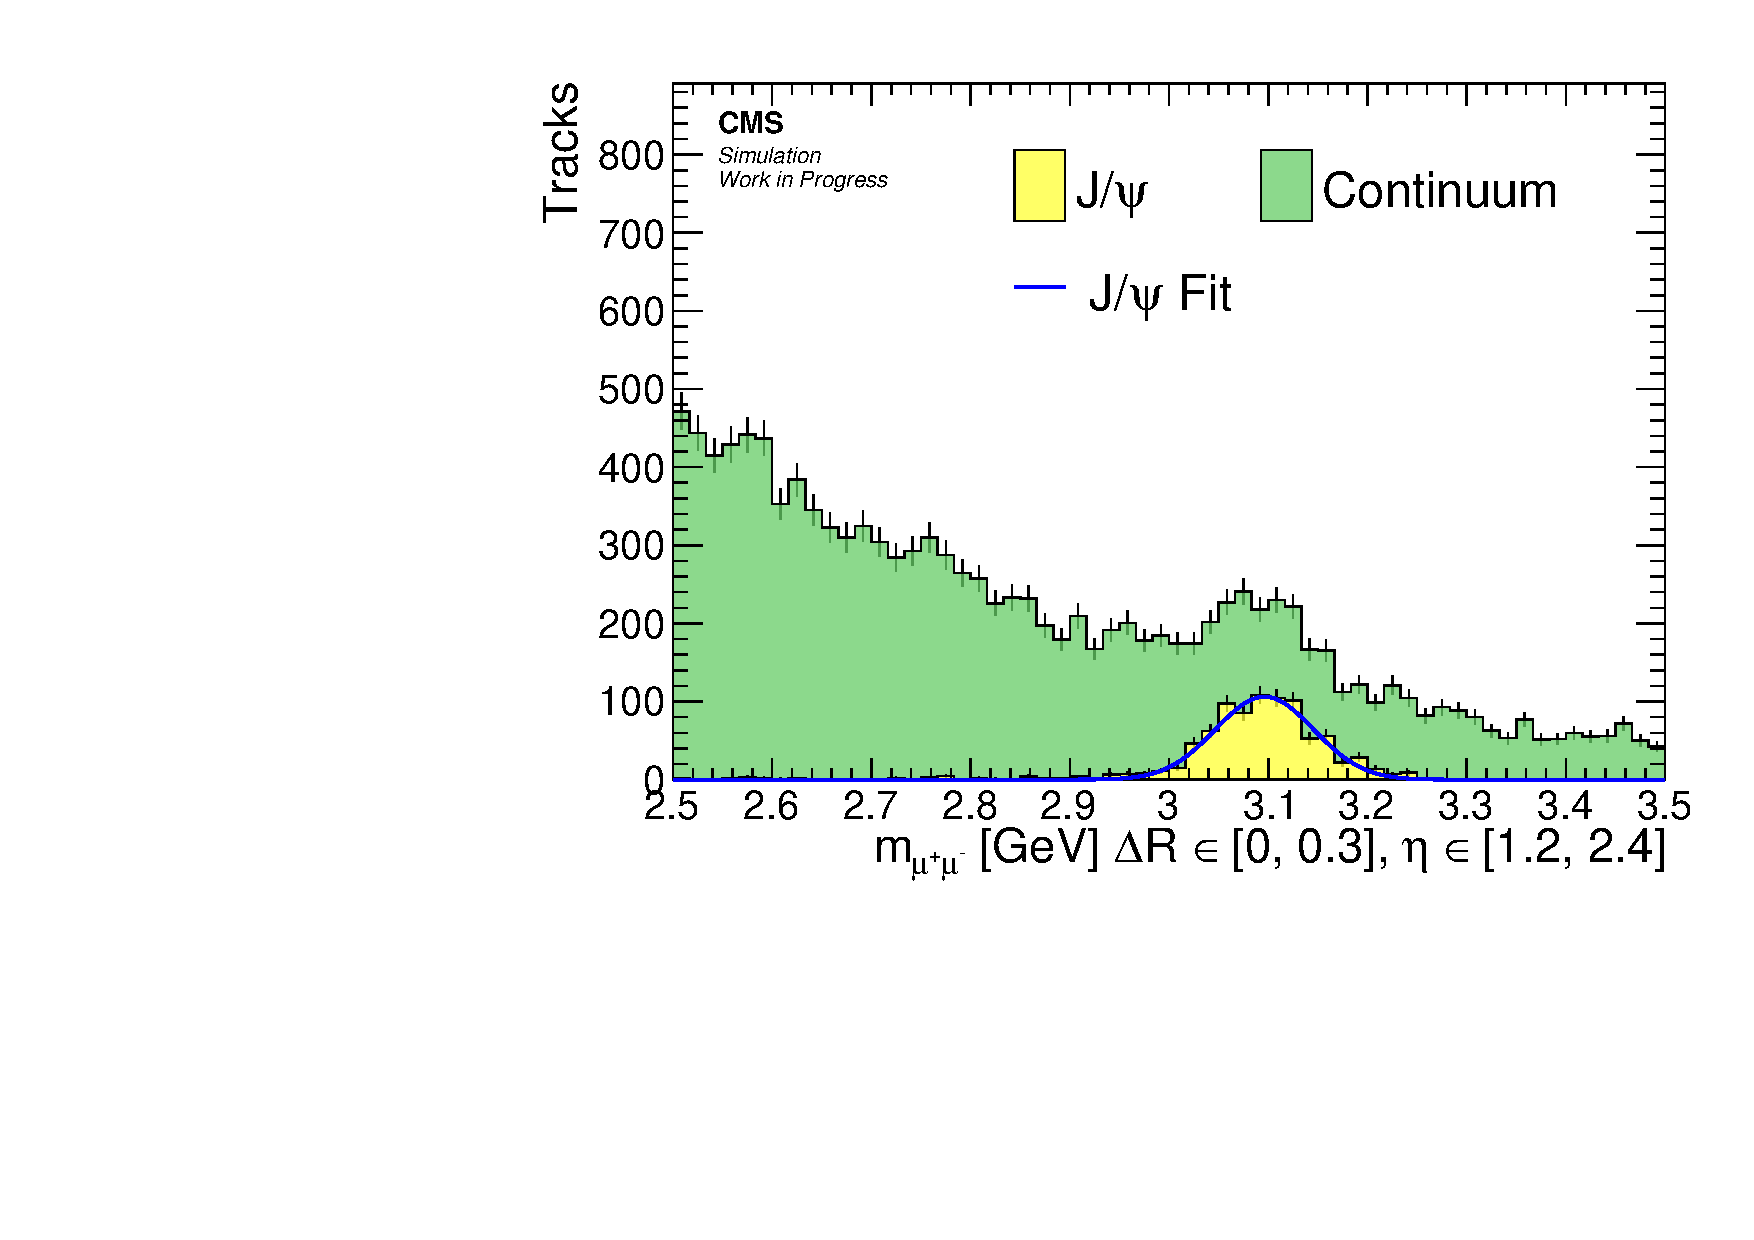
\includegraphics[width=0.32\linewidth]{plots/jpsi_muons_fit_bg_delta_r_single_electron/none_invMass_0_0.3_1.2_2.4.pdf} \,
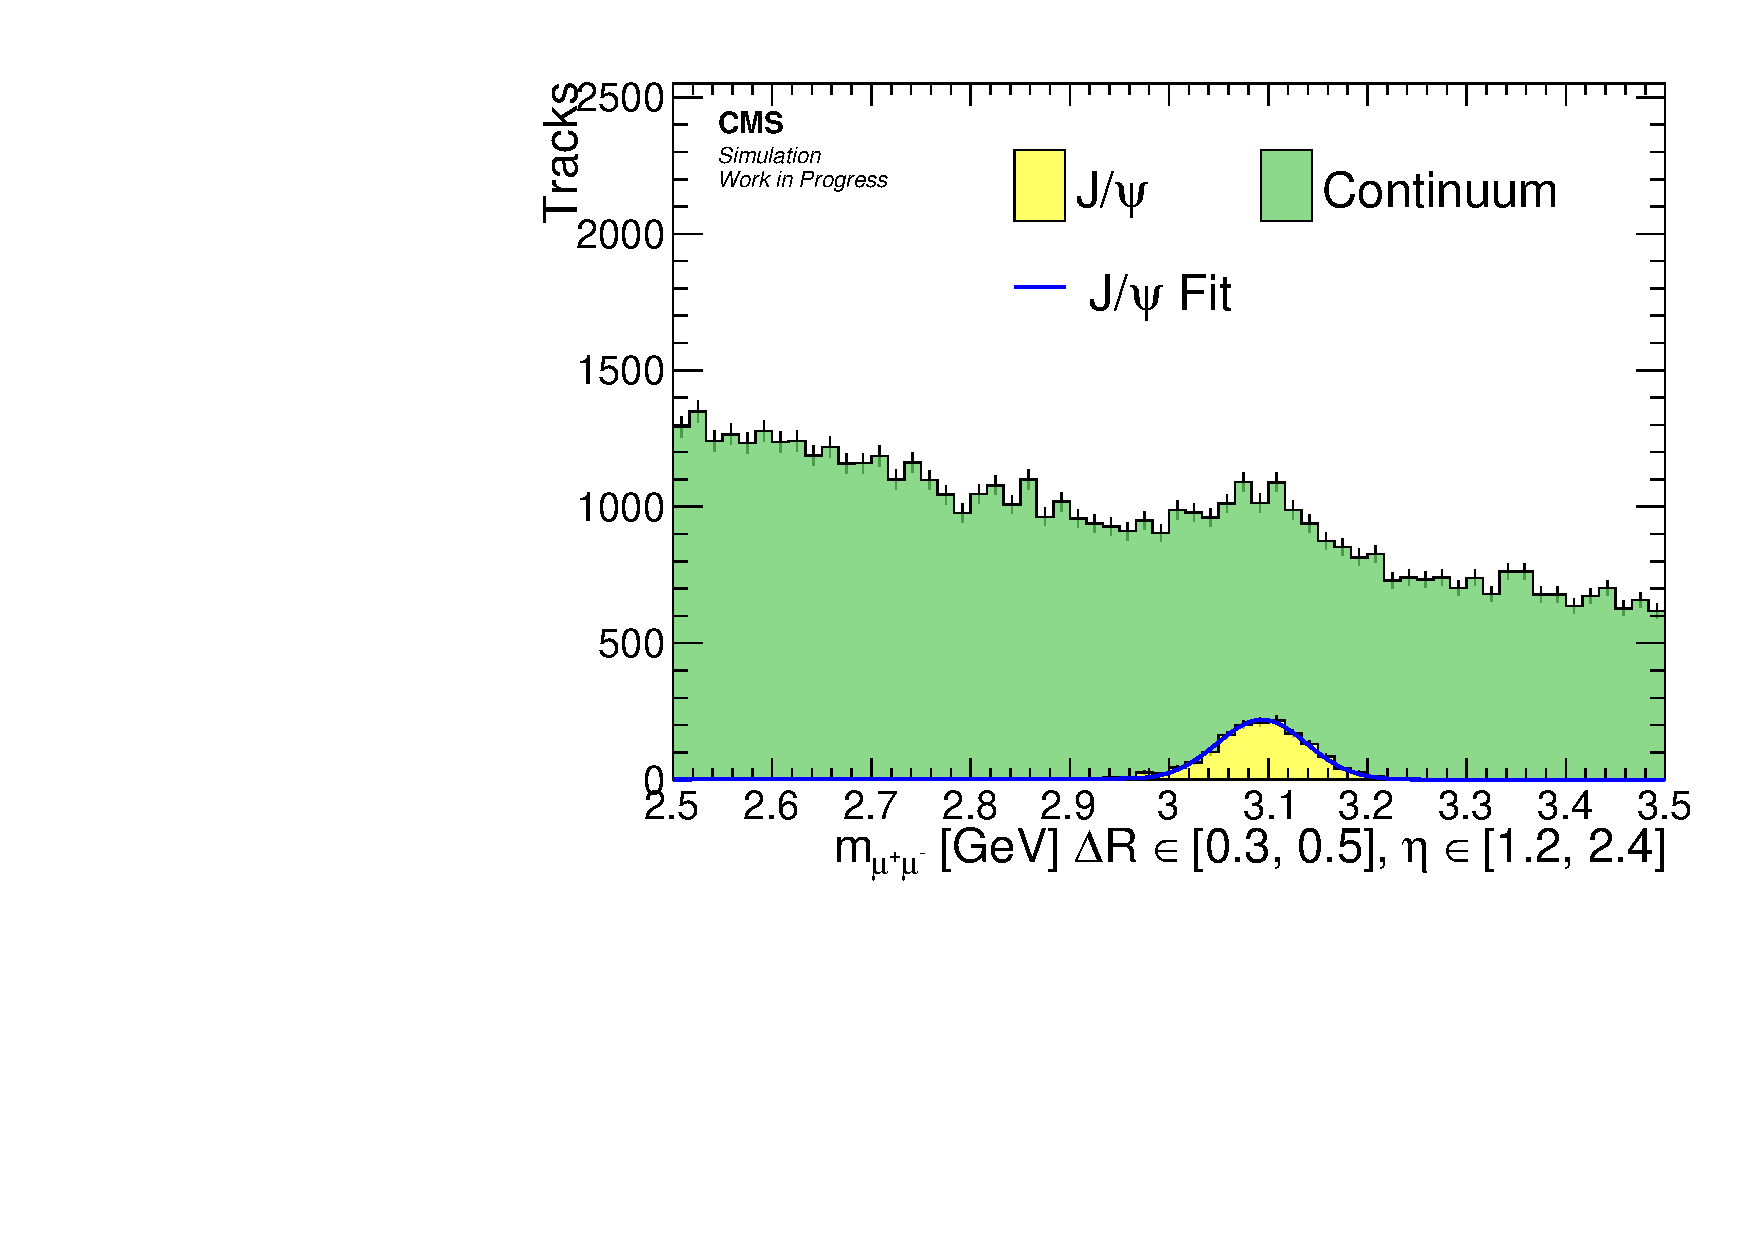
\includegraphics[width=0.32\linewidth]{plots/jpsi_muons_fit_bg_delta_r_single_electron/none_invMass_0.3_0.5_1.2_2.4.pdf} \,
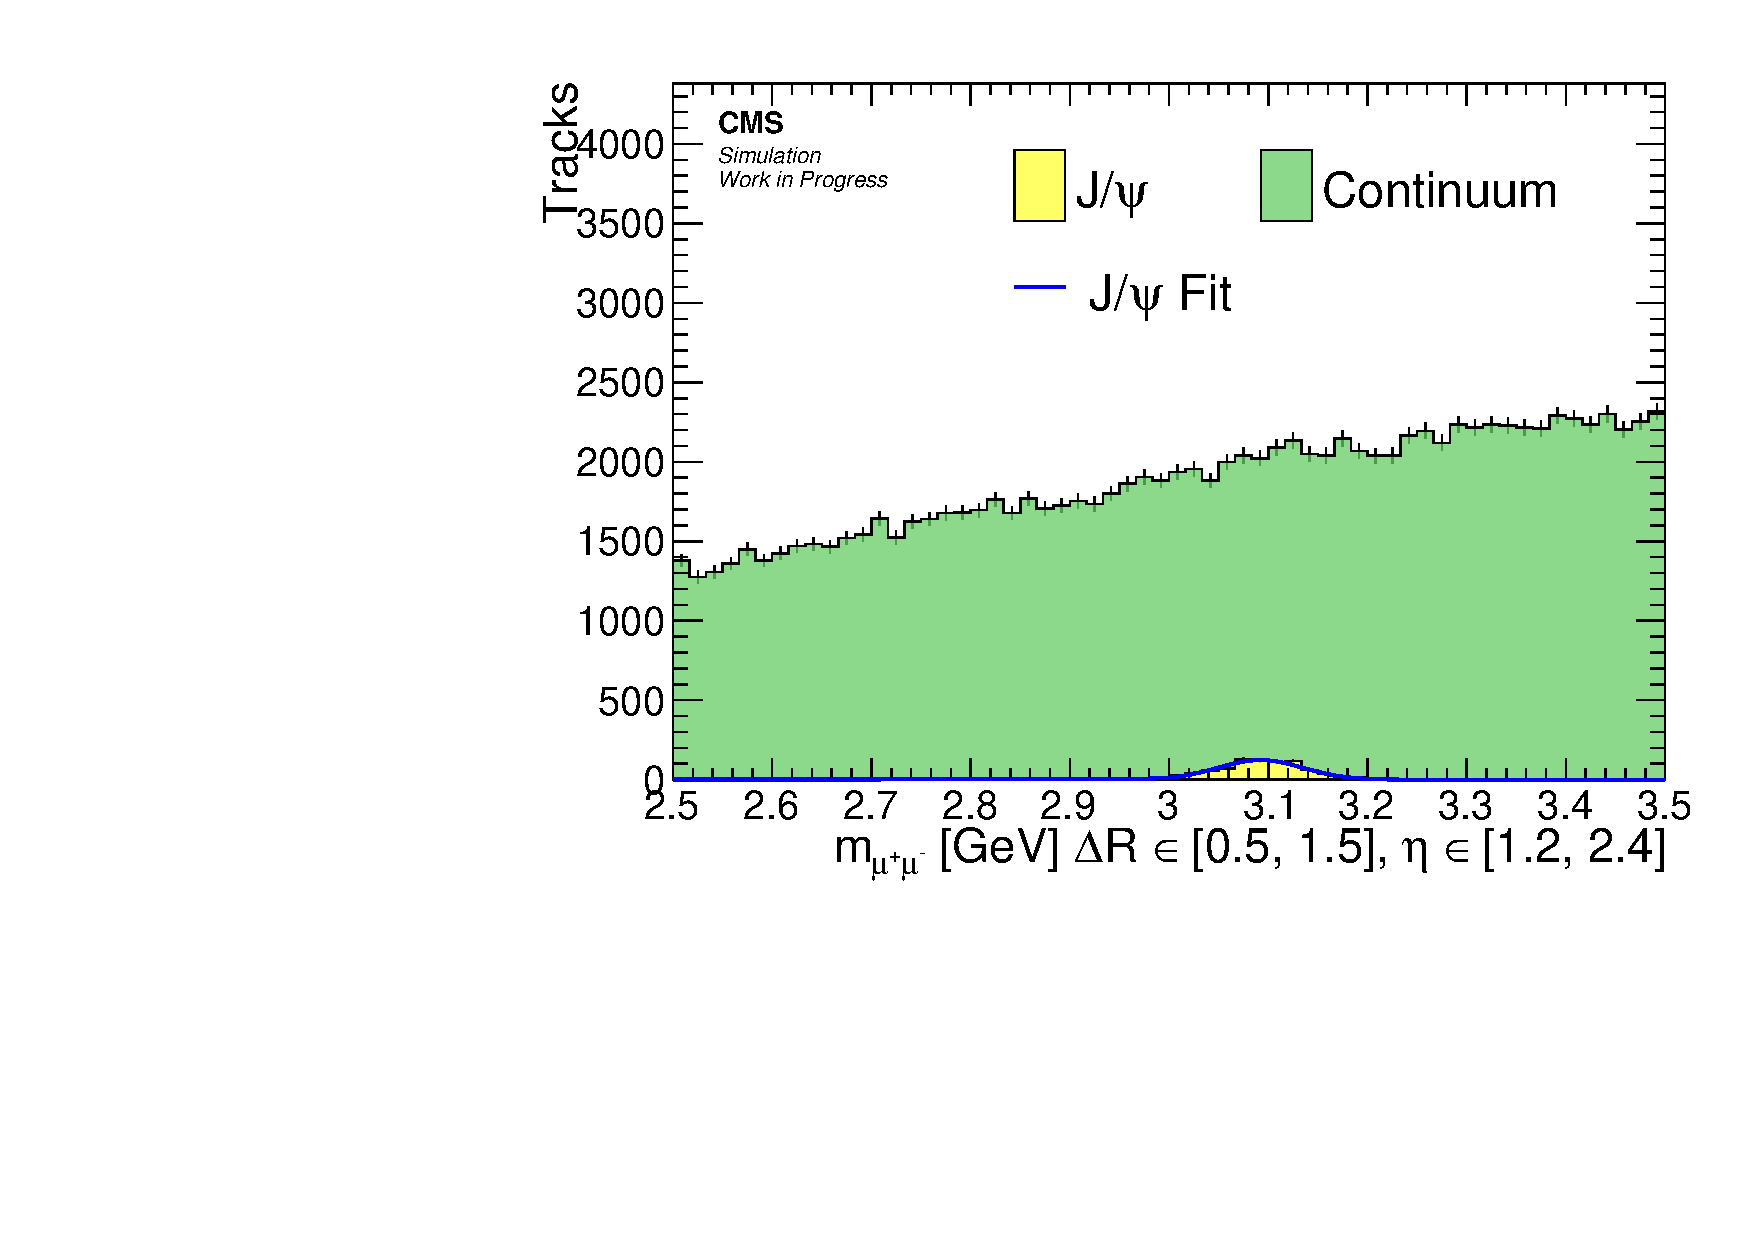
\includegraphics[width=0.32\linewidth]{plots/jpsi_muons_fit_bg_delta_r_single_electron/none_invMass_0.5_1.5_1.2_2.4.pdf} \\
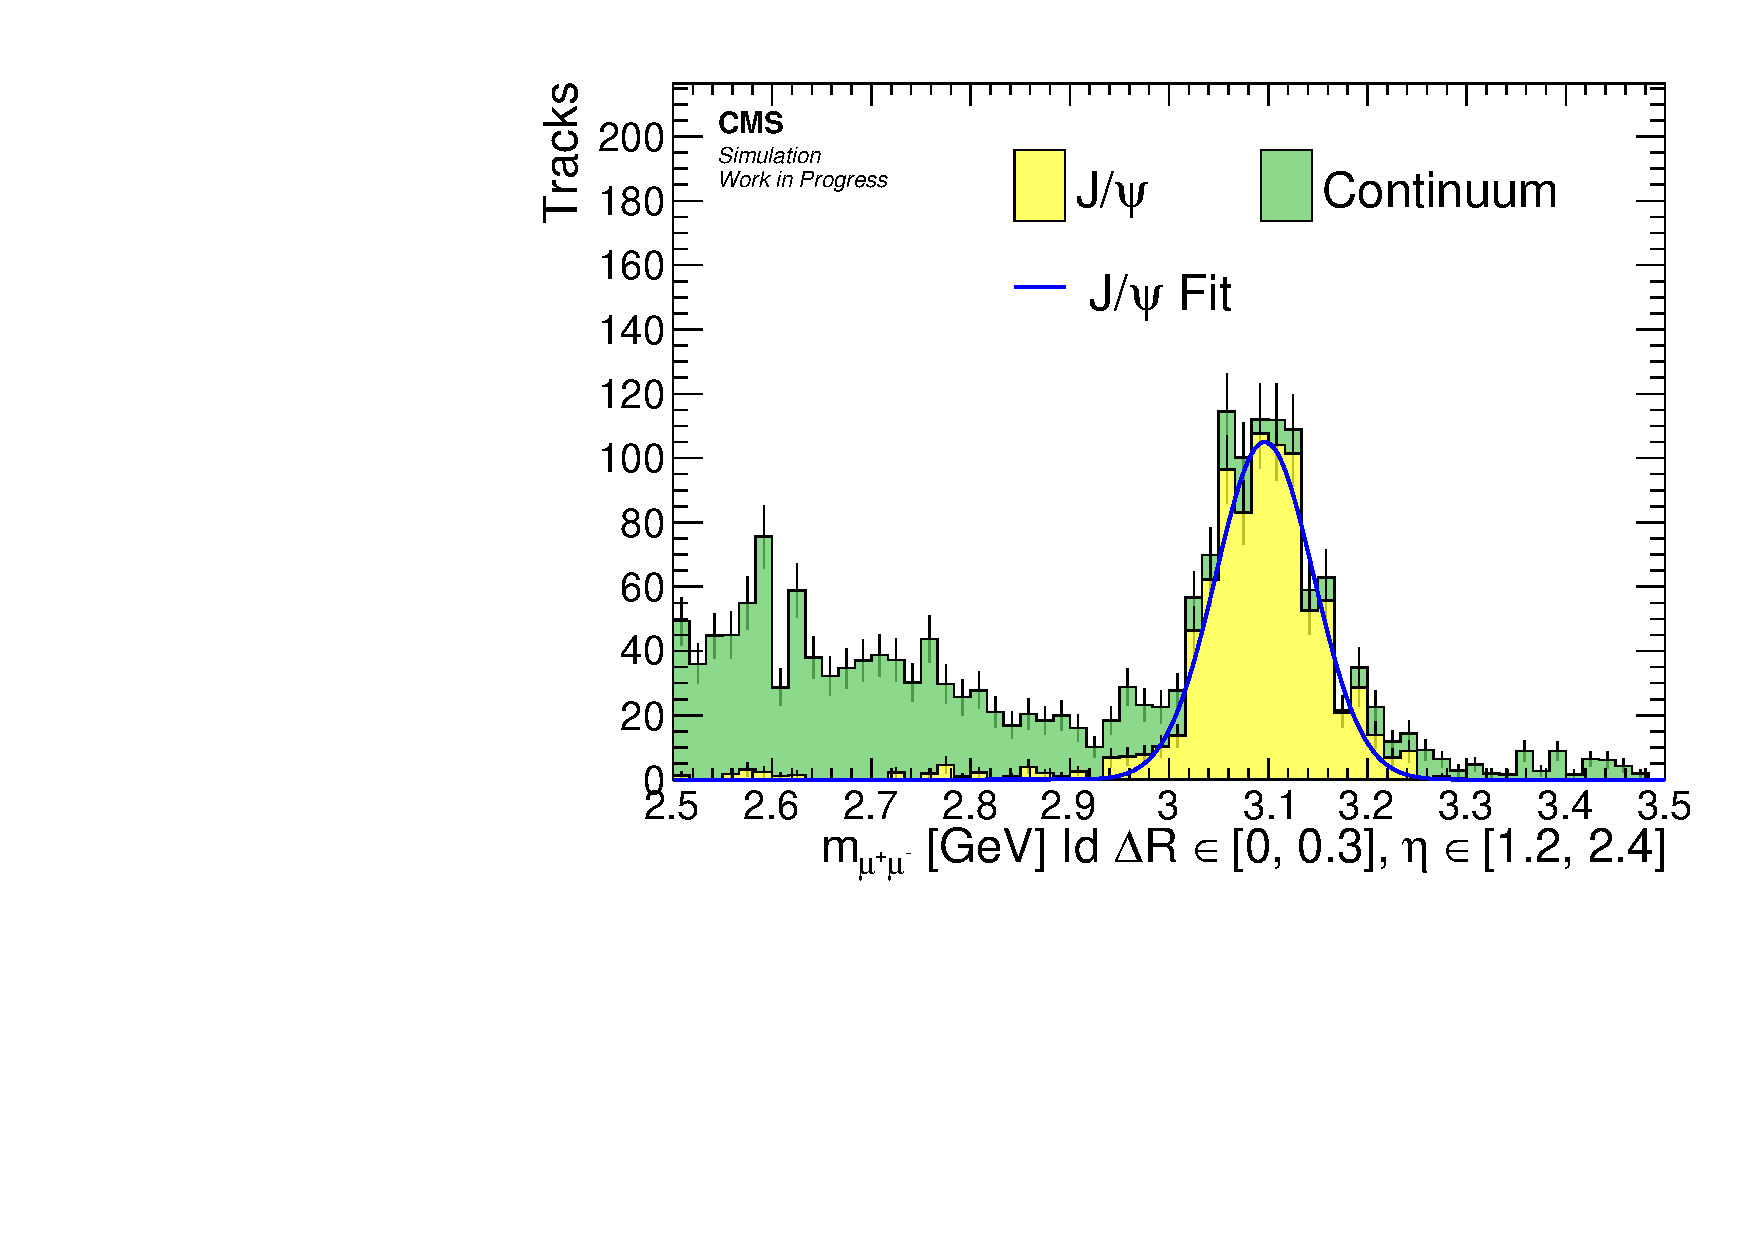
\includegraphics[width=0.32\linewidth]{plots/jpsi_muons_fit_bg_delta_r_single_electron/none_id_invMass_0_0.3_1.2_2.4.pdf} \,
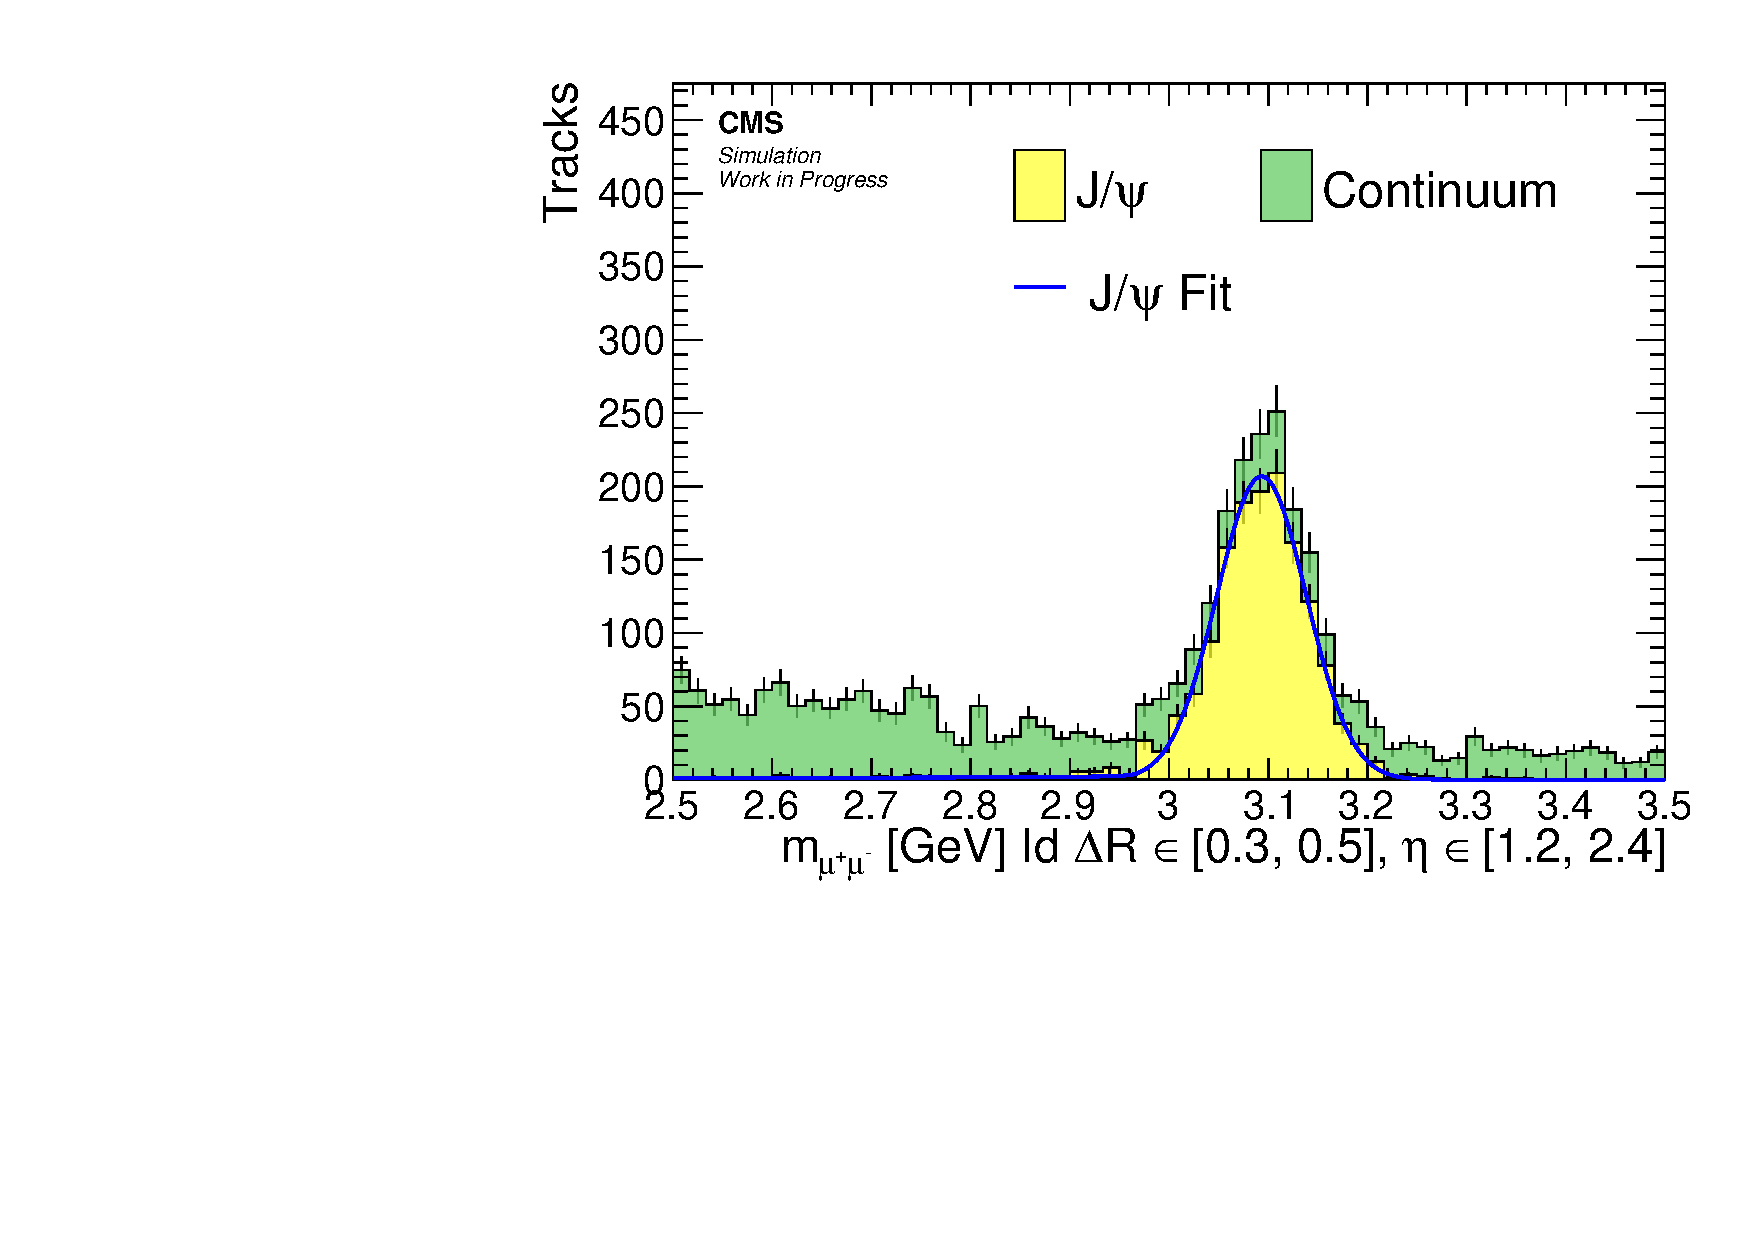
\includegraphics[width=0.32\linewidth]{plots/jpsi_muons_fit_bg_delta_r_single_electron/none_id_invMass_0.3_0.5_1.2_2.4.pdf} \,
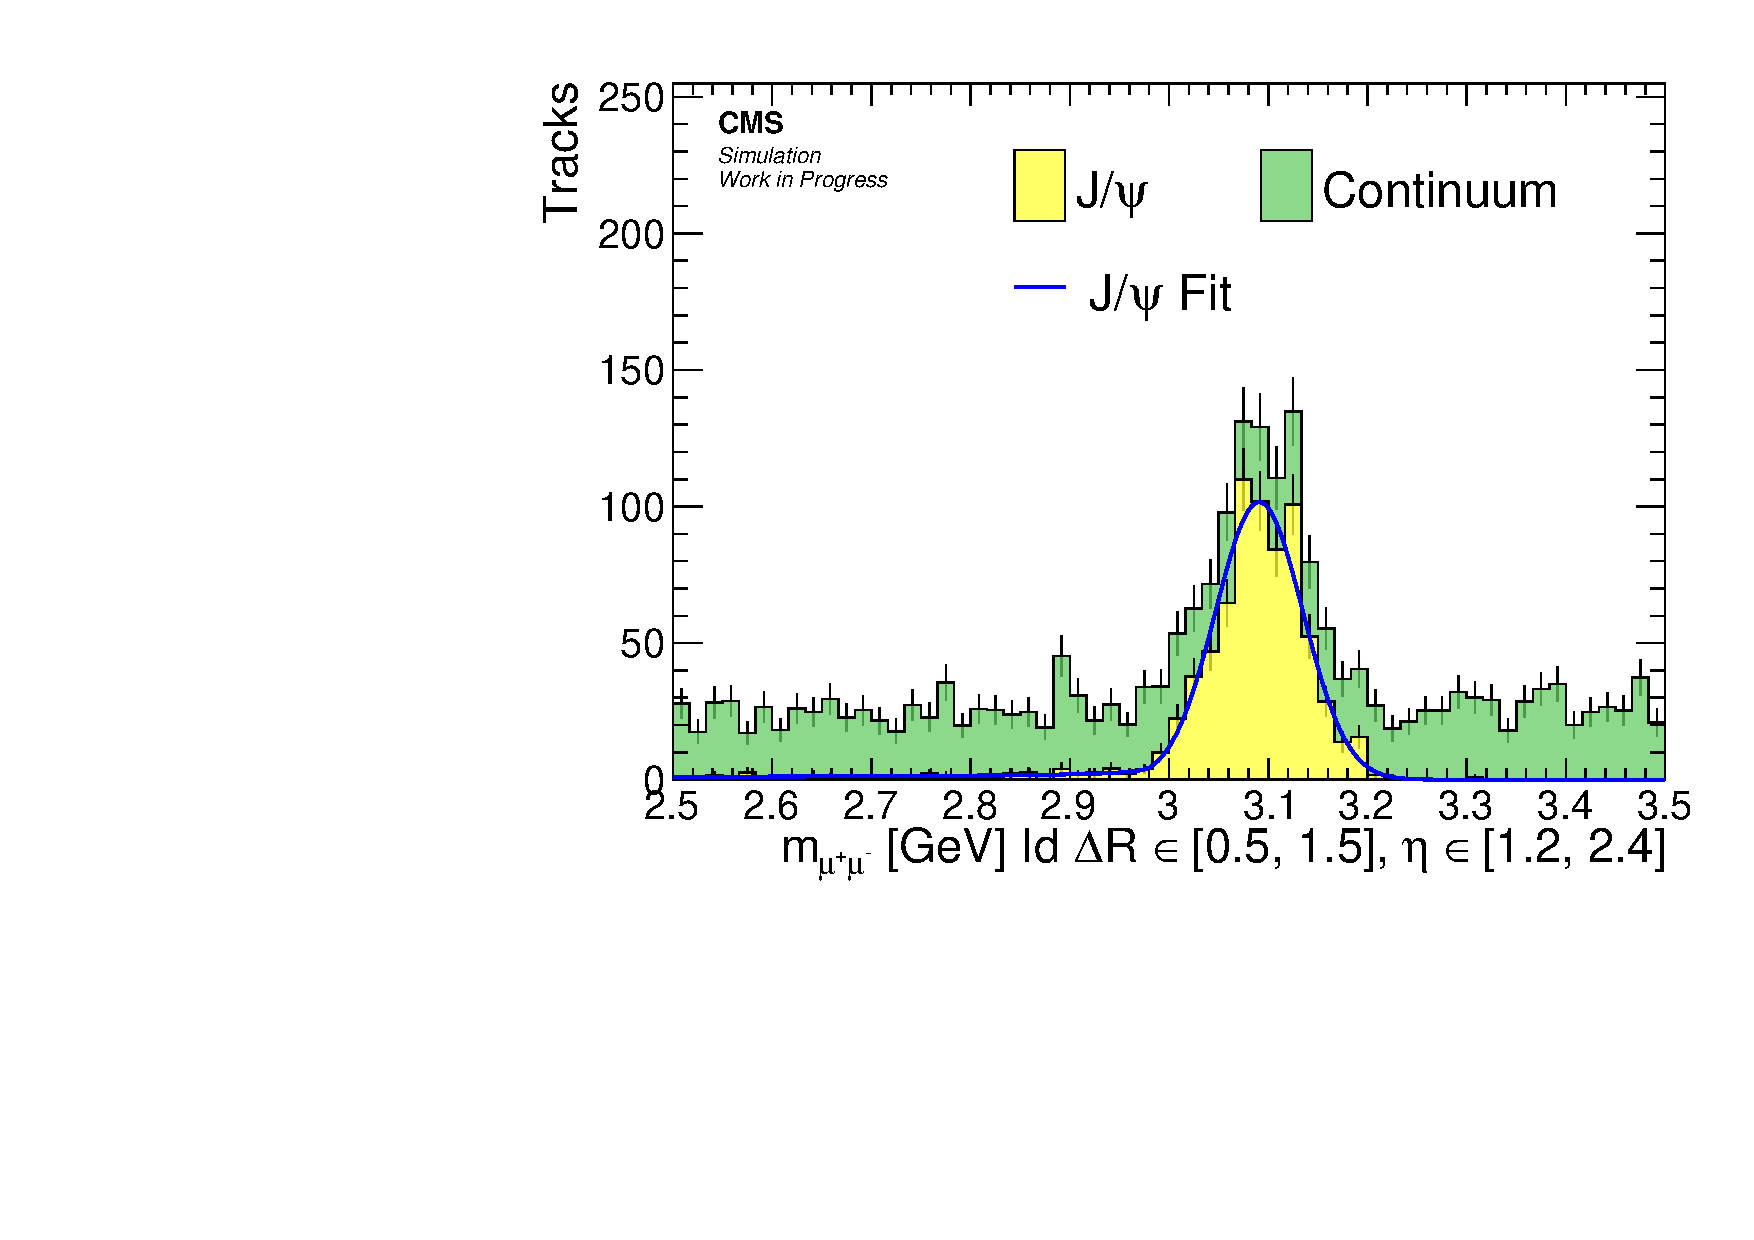
\includegraphics[width=0.32\linewidth]{plots/jpsi_muons_fit_bg_delta_r_single_electron/none_id_invMass_0.5_1.5_1.2_2.4.pdf}  \\
\caption[Simluation endcaps muons fits]{Simluation endcaps muons fits for denominator (top) and numerator (bottom) for $0<\DR<0.3$  (left), $0.3<\DR<0.5$ (center), $0.5<\DR<1.5$ (right)}
\label{fig:tb-endcaps-simulation}
\end{figure}

\begin{figure}[!htbp]
\centering
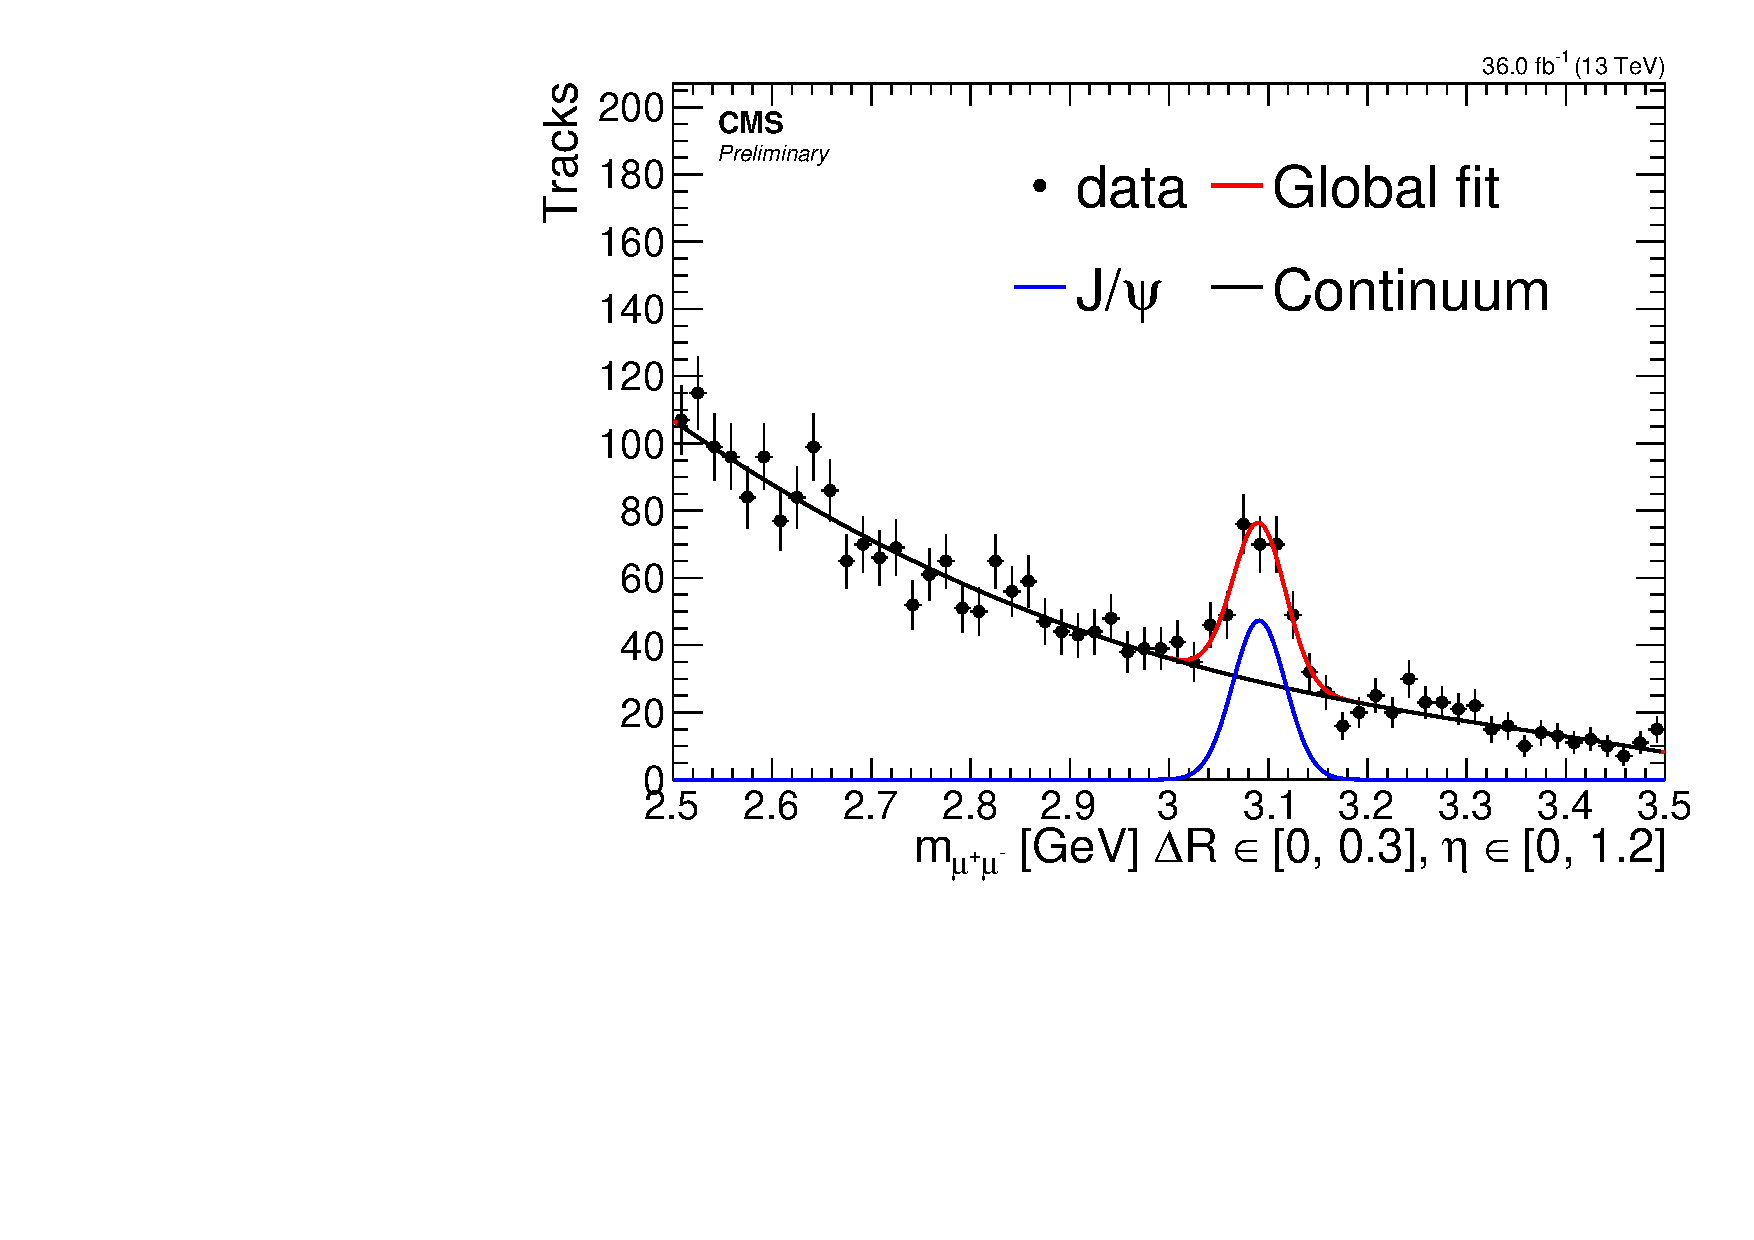
\includegraphics[width=0.32\linewidth]{plots/jpsi_muons_fit_data_delta_r_single_electron/none_invMass_0_0.3_0_1.2.pdf} \,
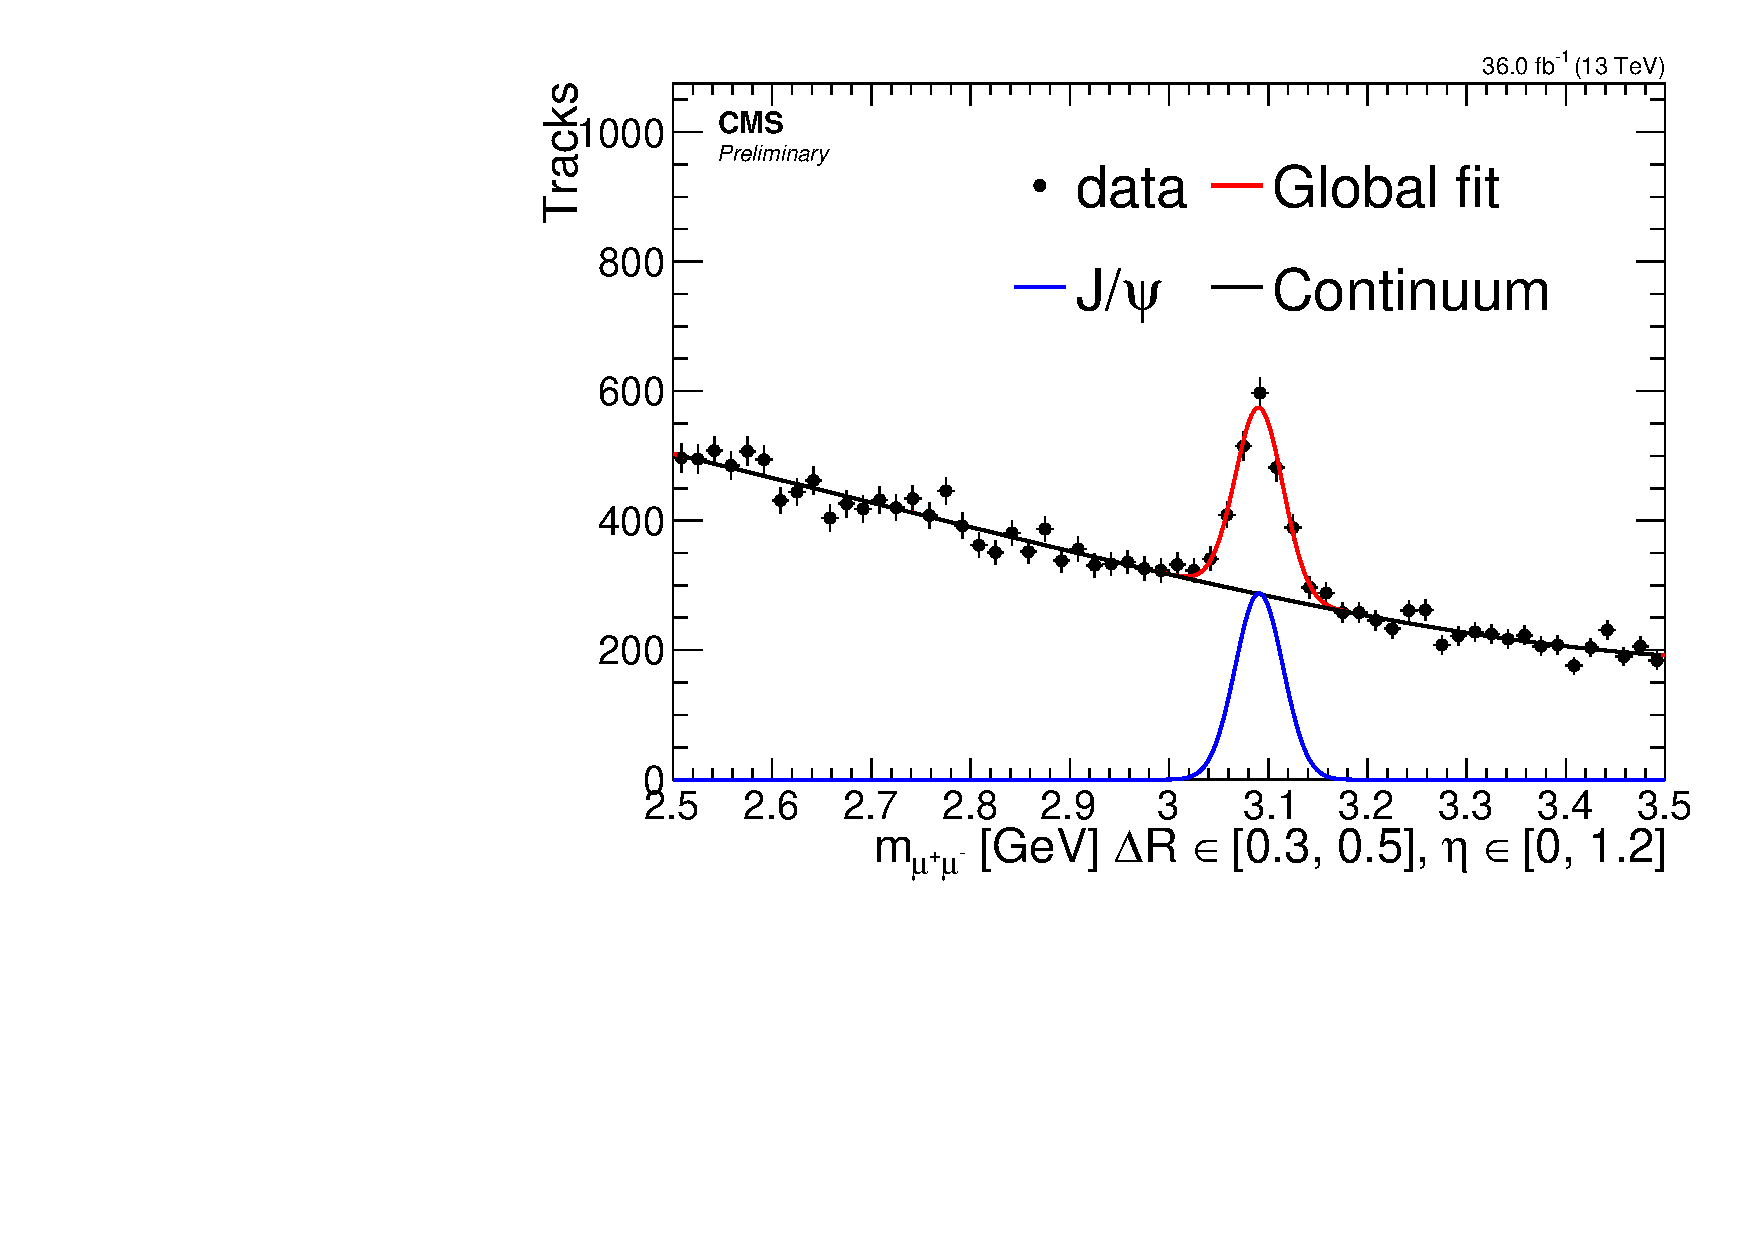
\includegraphics[width=0.32\linewidth]{plots/jpsi_muons_fit_data_delta_r_single_electron/none_invMass_0.3_0.5_0_1.2.pdf}  \,
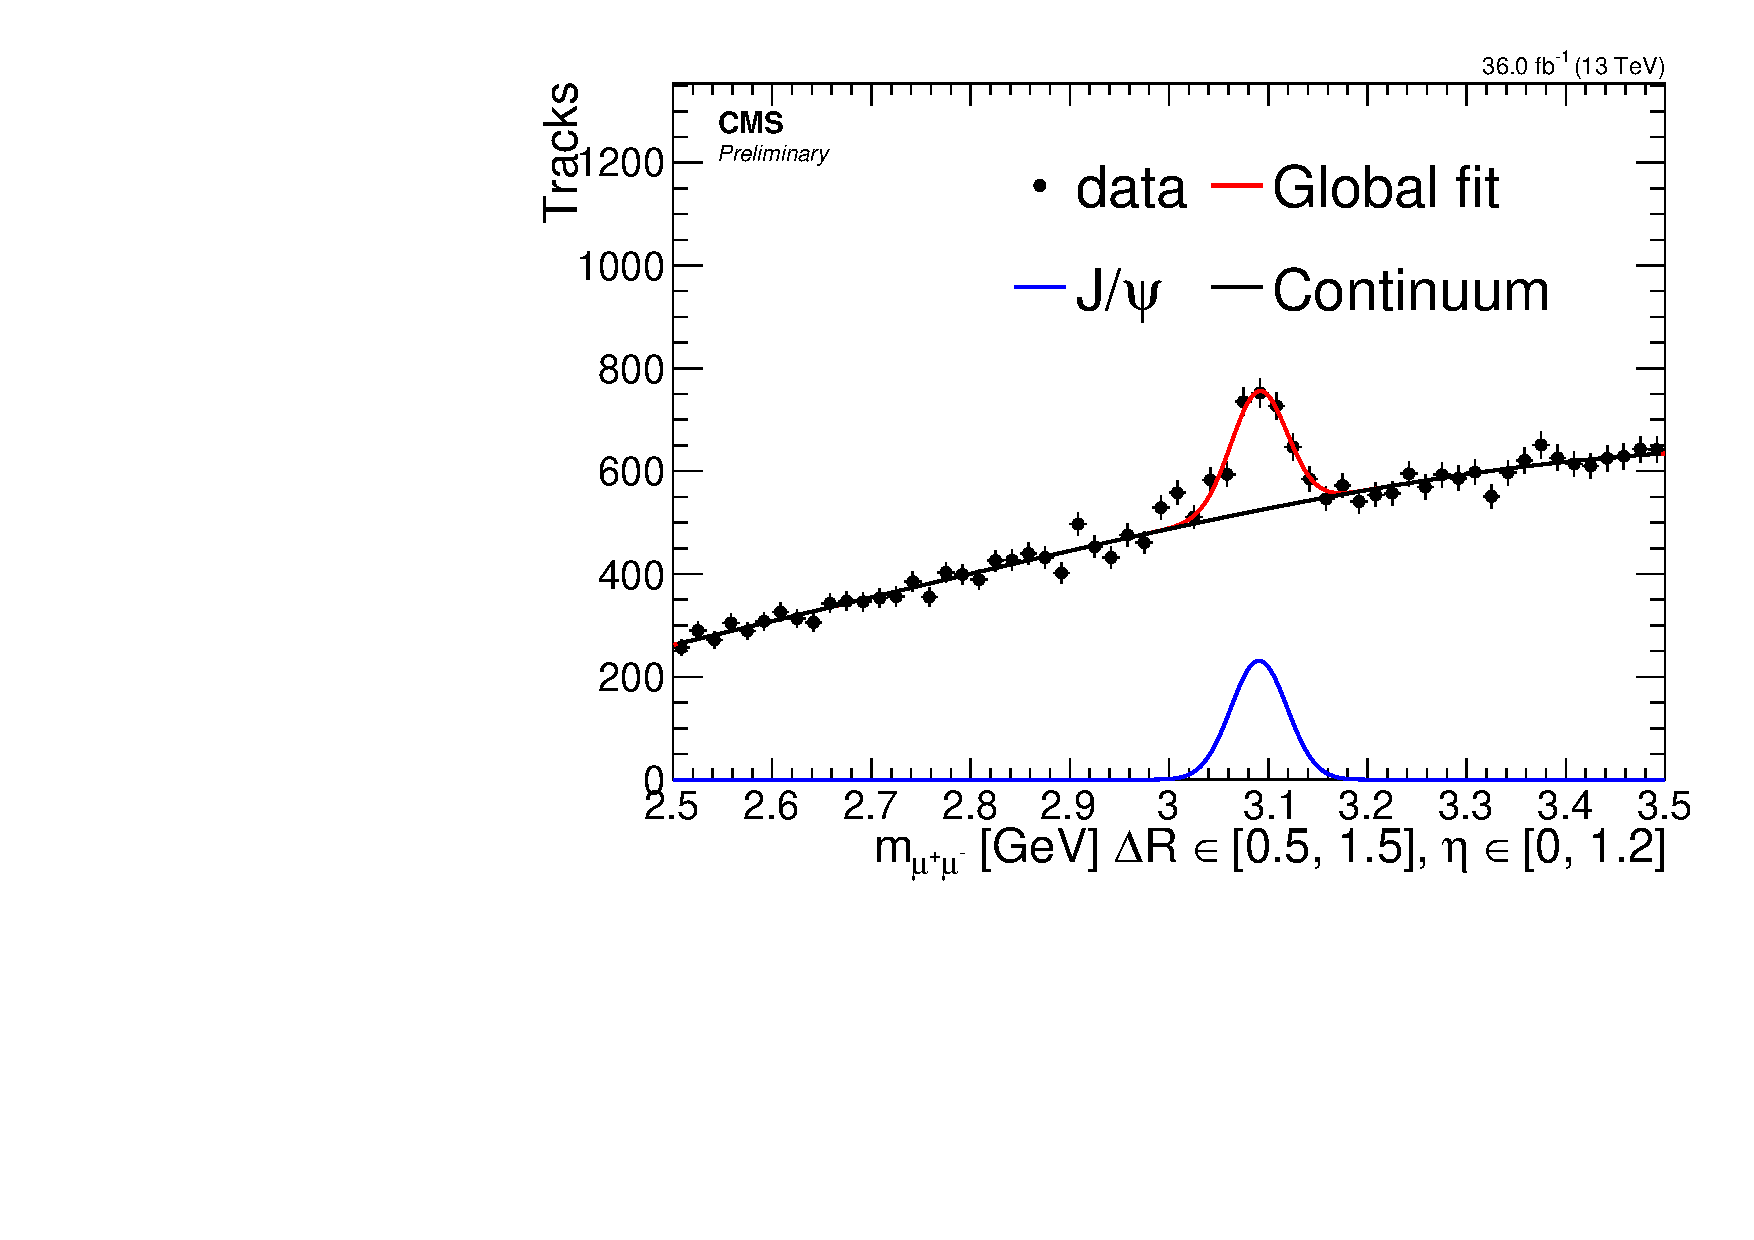
\includegraphics[width=0.32\linewidth]{plots/jpsi_muons_fit_data_delta_r_single_electron/none_invMass_0.5_1.5_0_1.2.pdf} \\
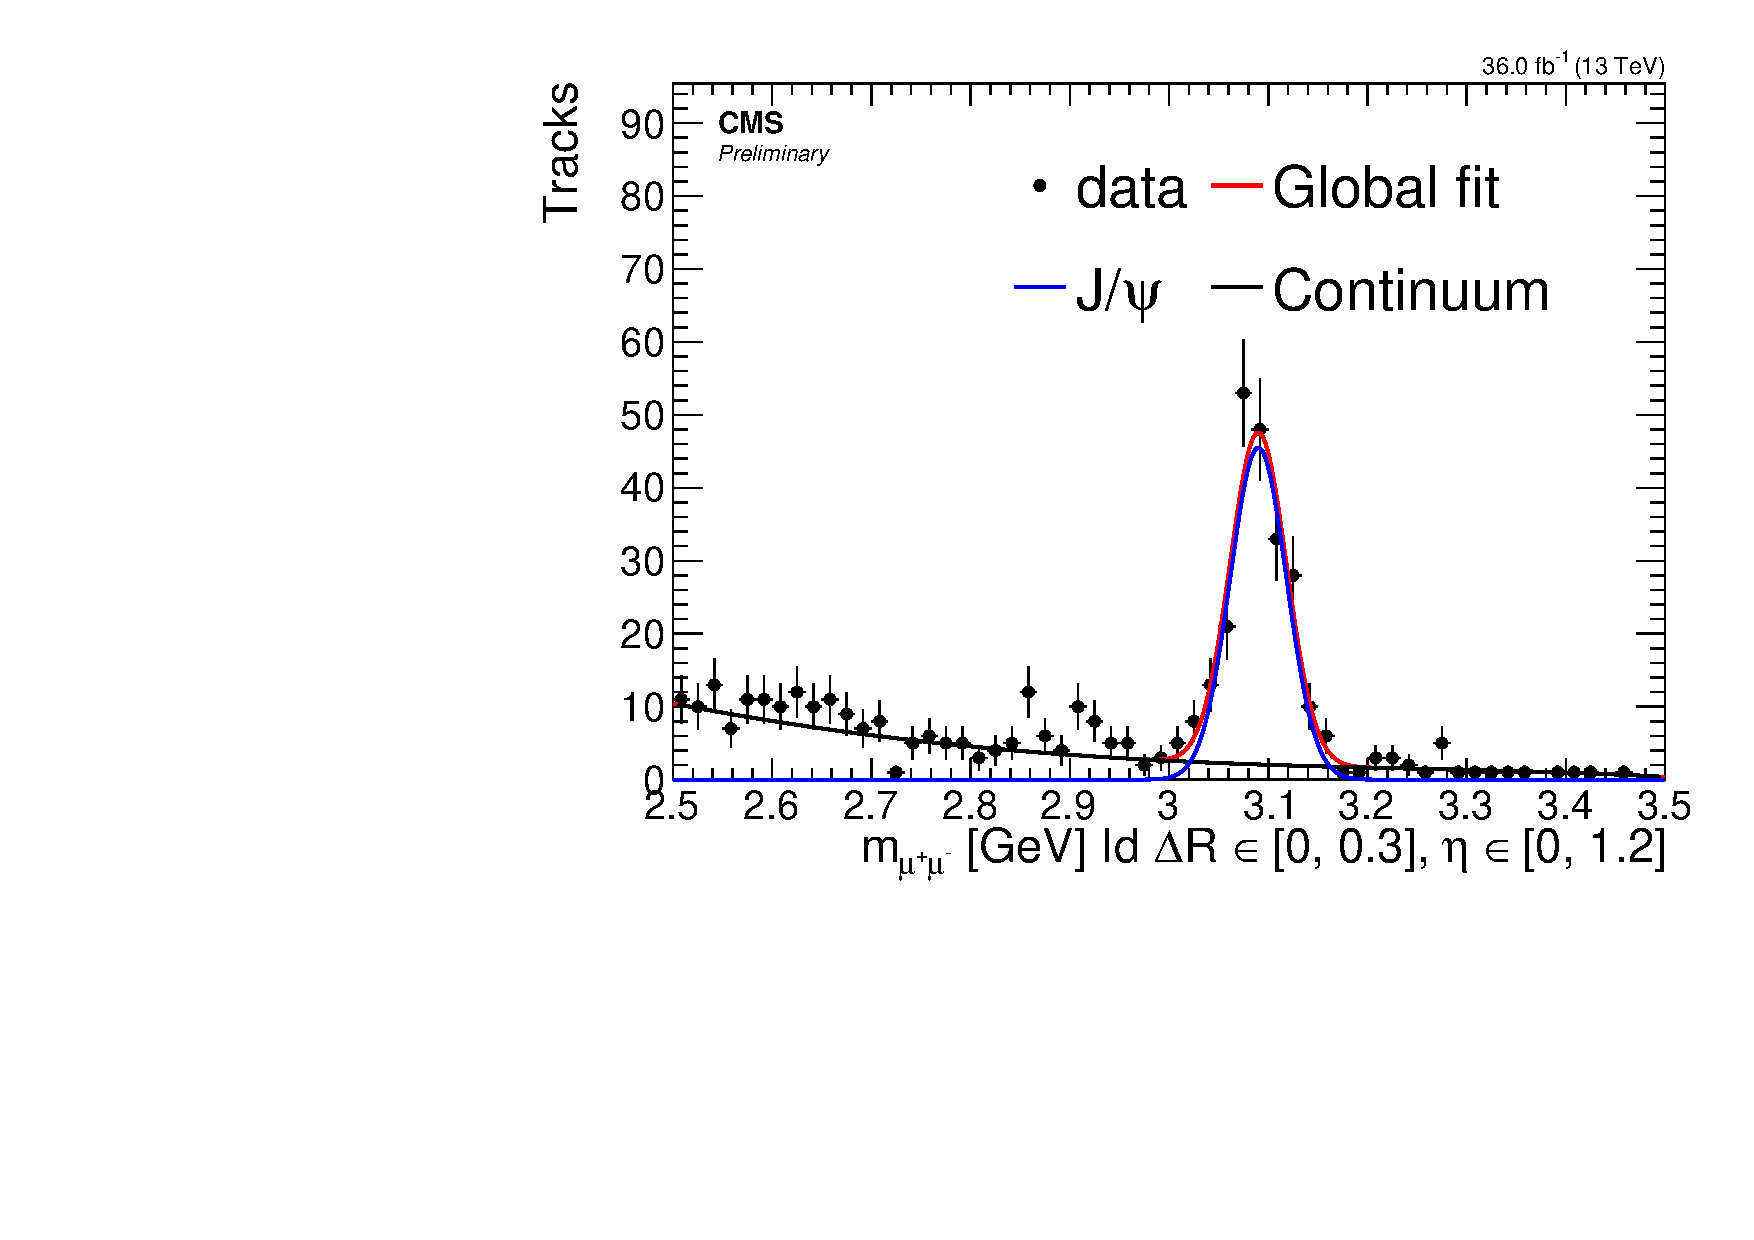
\includegraphics[width=0.32\linewidth]{plots/jpsi_muons_fit_data_delta_r_single_electron/none_id_invMass_0_0.3_0_1.2.pdf} \,
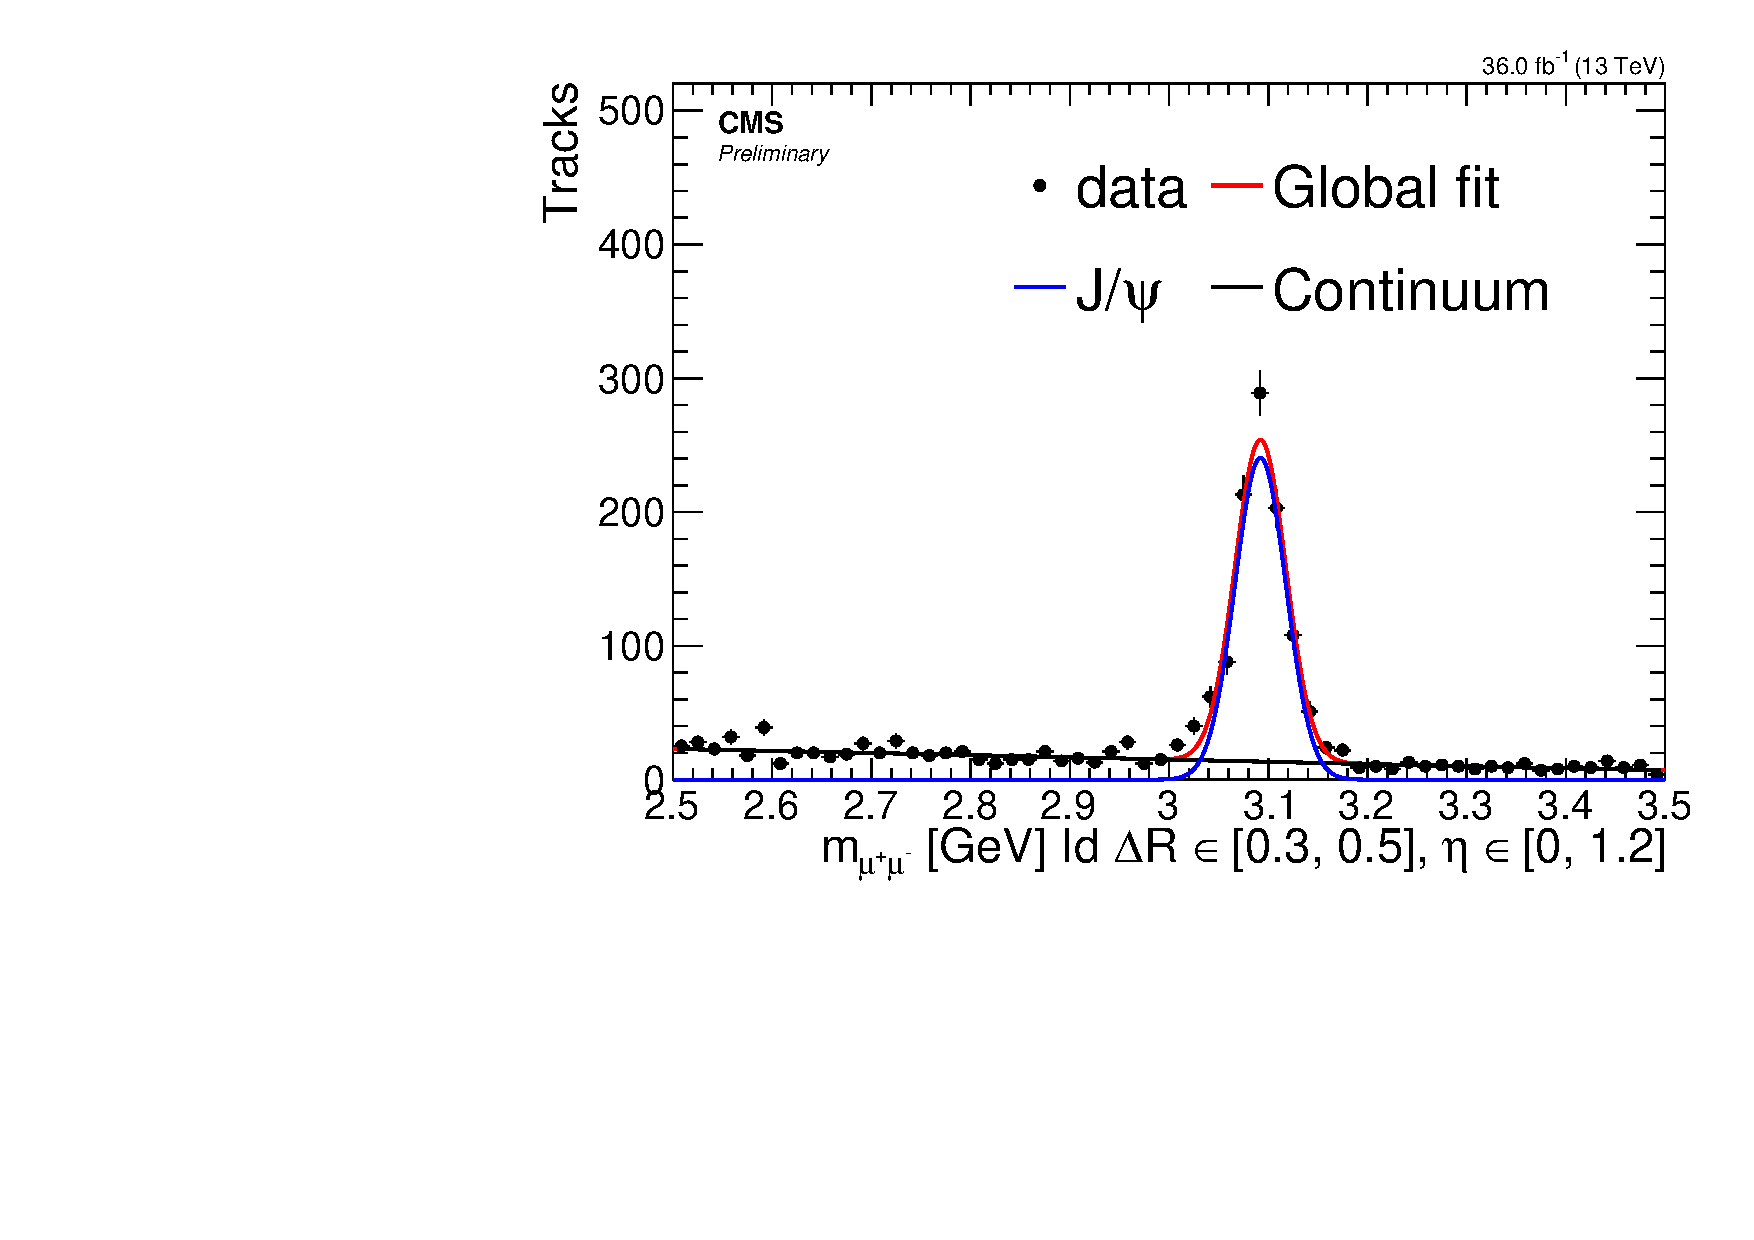
\includegraphics[width=0.32\linewidth]{plots/jpsi_muons_fit_data_delta_r_single_electron/none_id_invMass_0.3_0.5_0_1.2.pdf}  \,
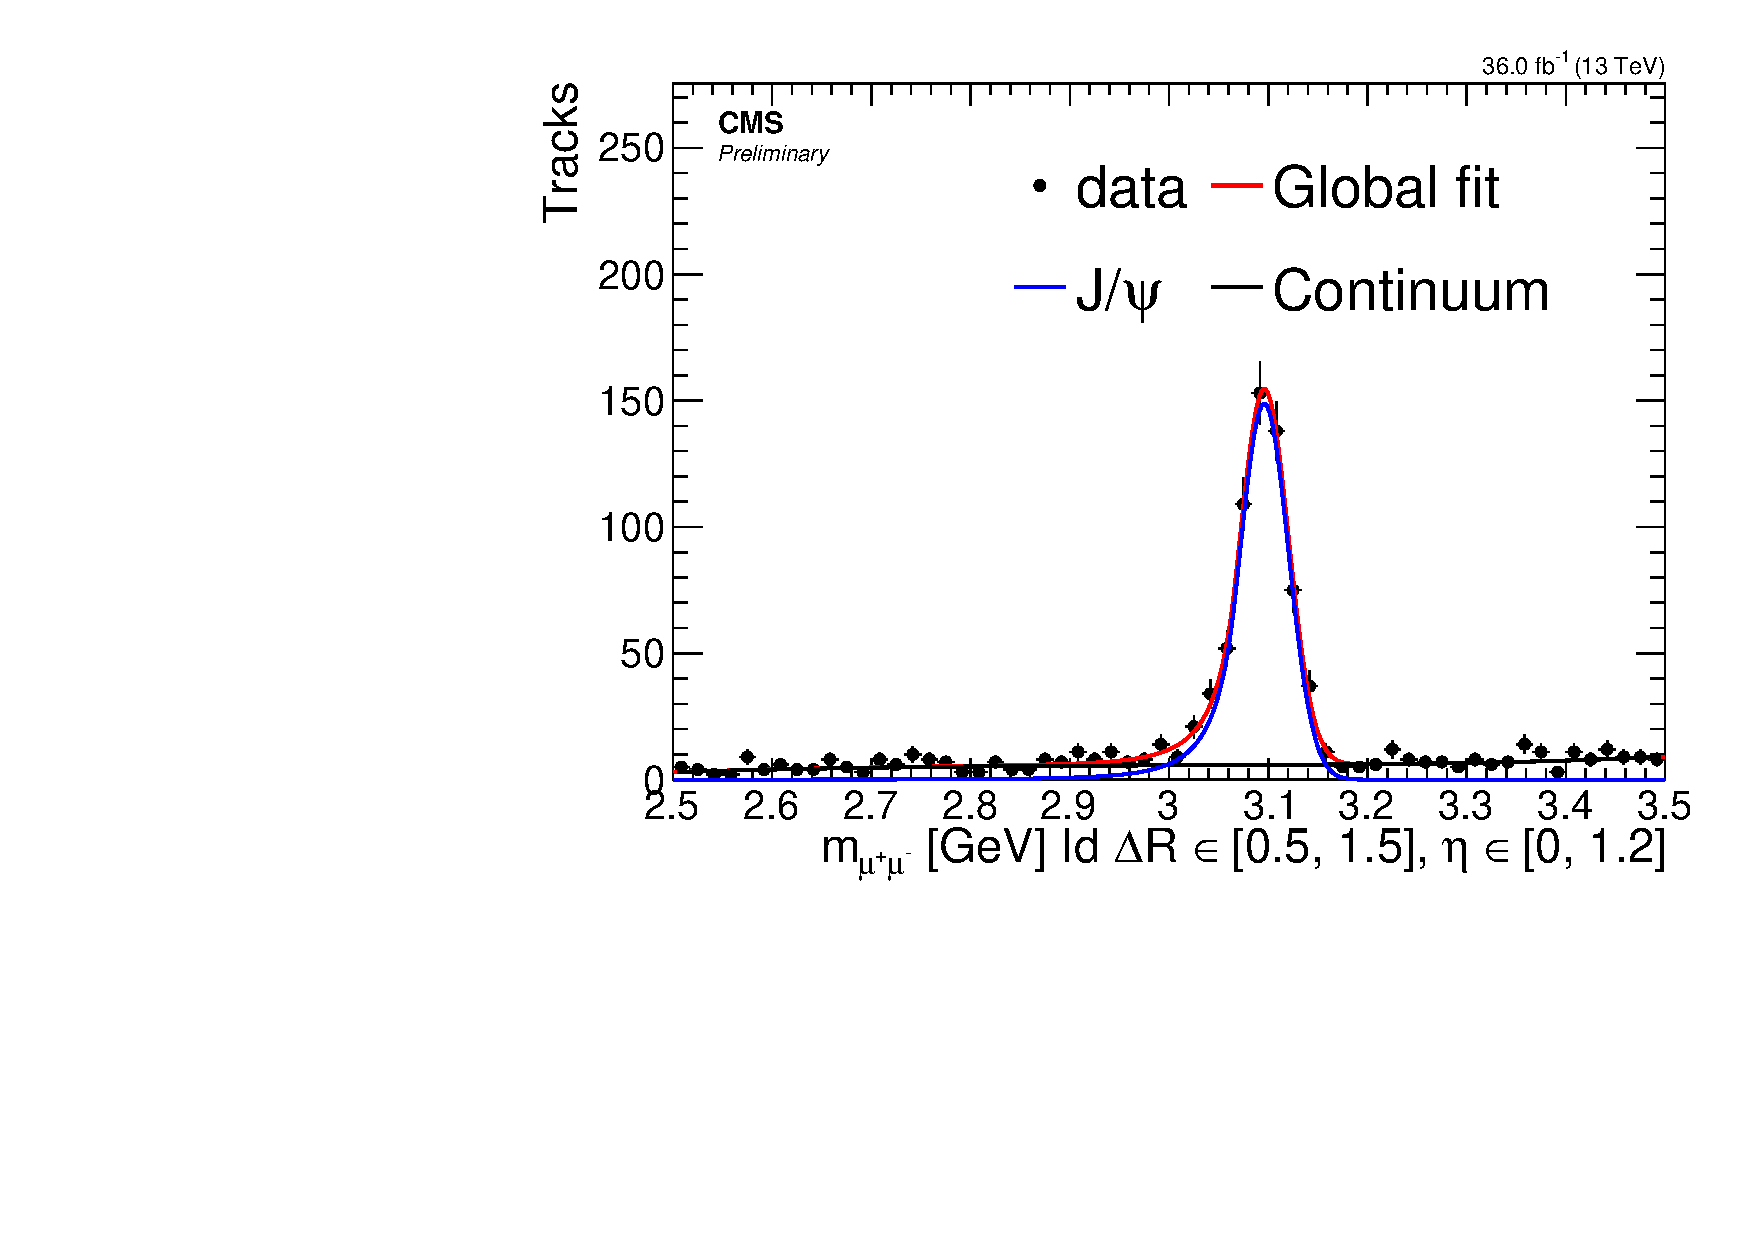
\includegraphics[width=0.32\linewidth]{plots/jpsi_muons_fit_data_delta_r_single_electron/none_id_invMass_0.5_1.5_0_1.2.pdf} \\
\caption[Data barrel muons fits]{Data barrel muons fits for denominator (top) and numerator (bottom) for $0<\DR<0.3$  (left), $0.3<\DR<0.5$ (center), $0.5<\DR<1.5$ (right)}
\label{fig:tb-barrel-data}
\end{figure}

\begin{figure}[!htbp]
\centering
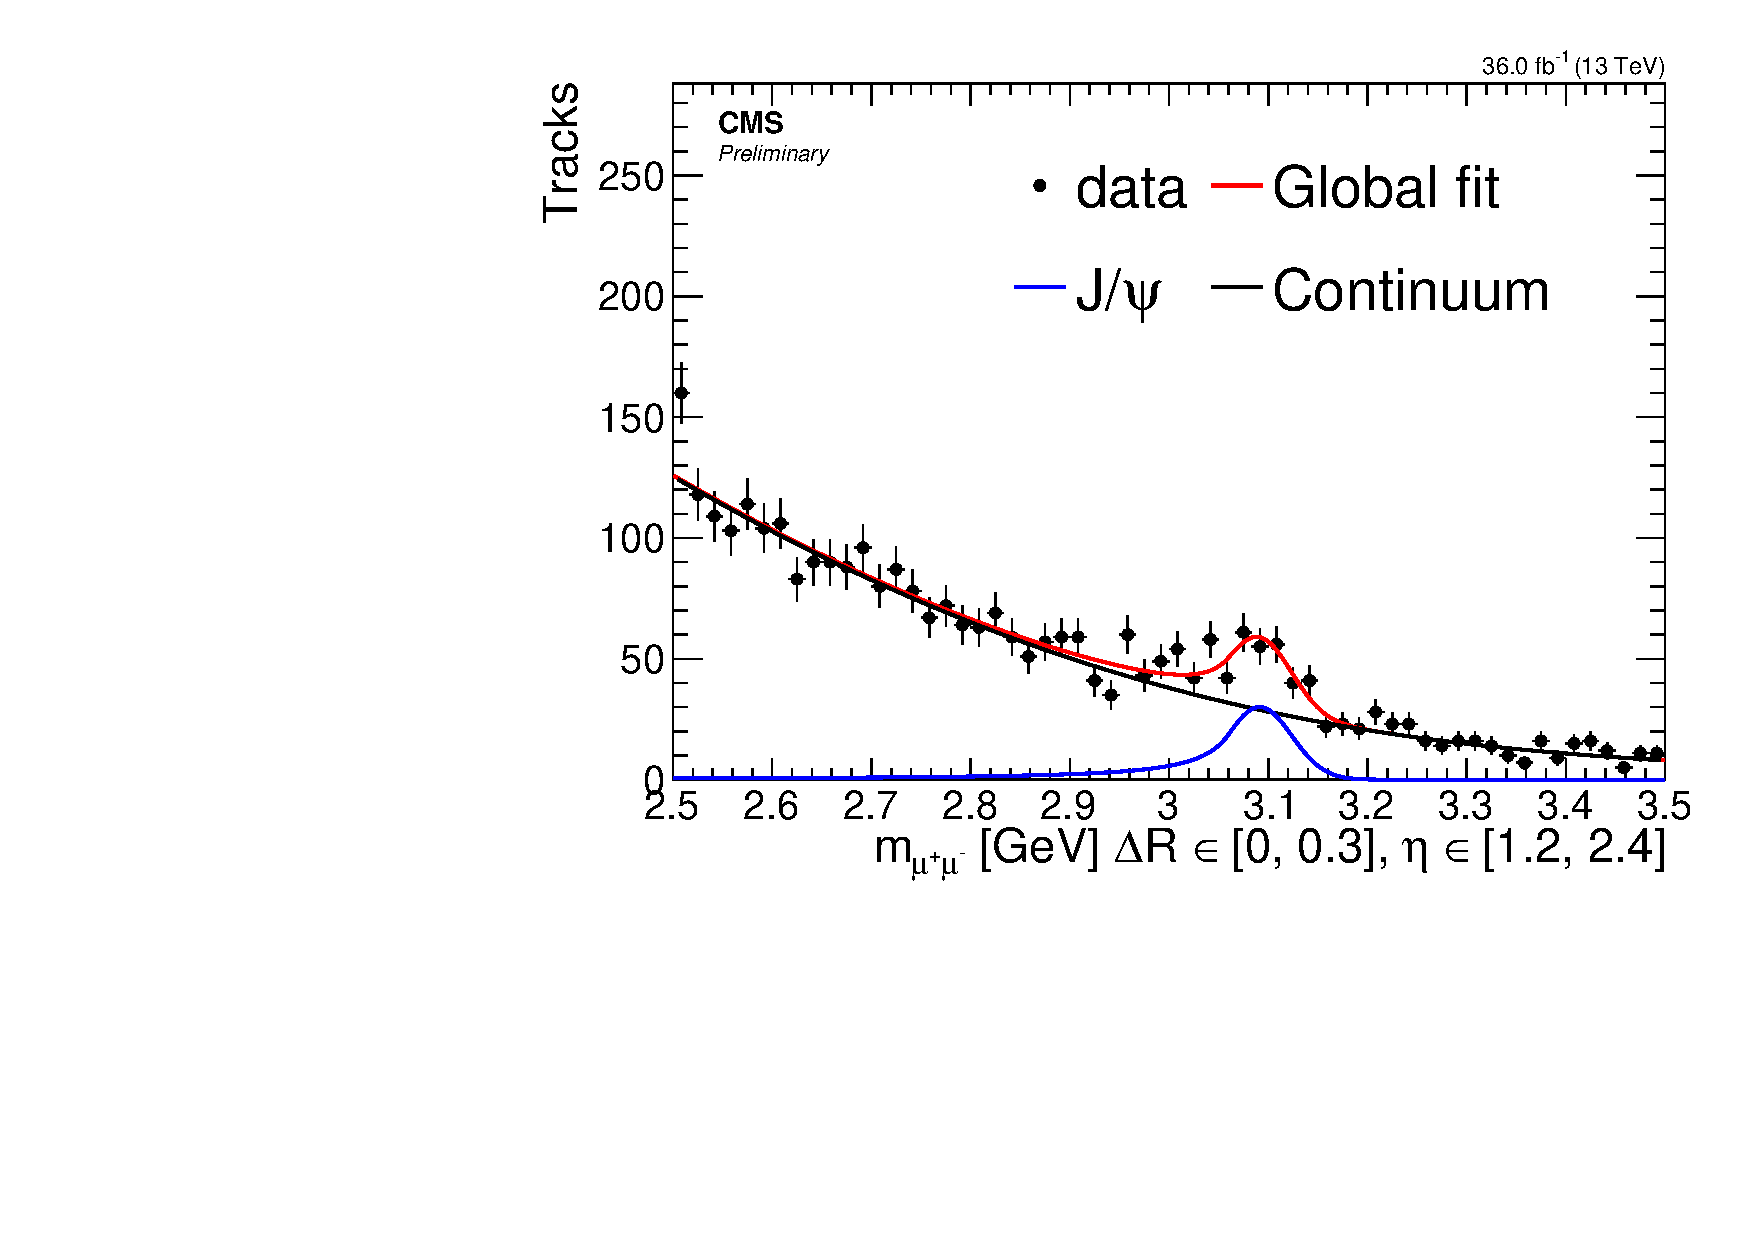
\includegraphics[width=0.32\linewidth]{plots/jpsi_muons_fit_data_delta_r_single_electron/none_invMass_0_0.3_1.2_2.4.pdf} \,
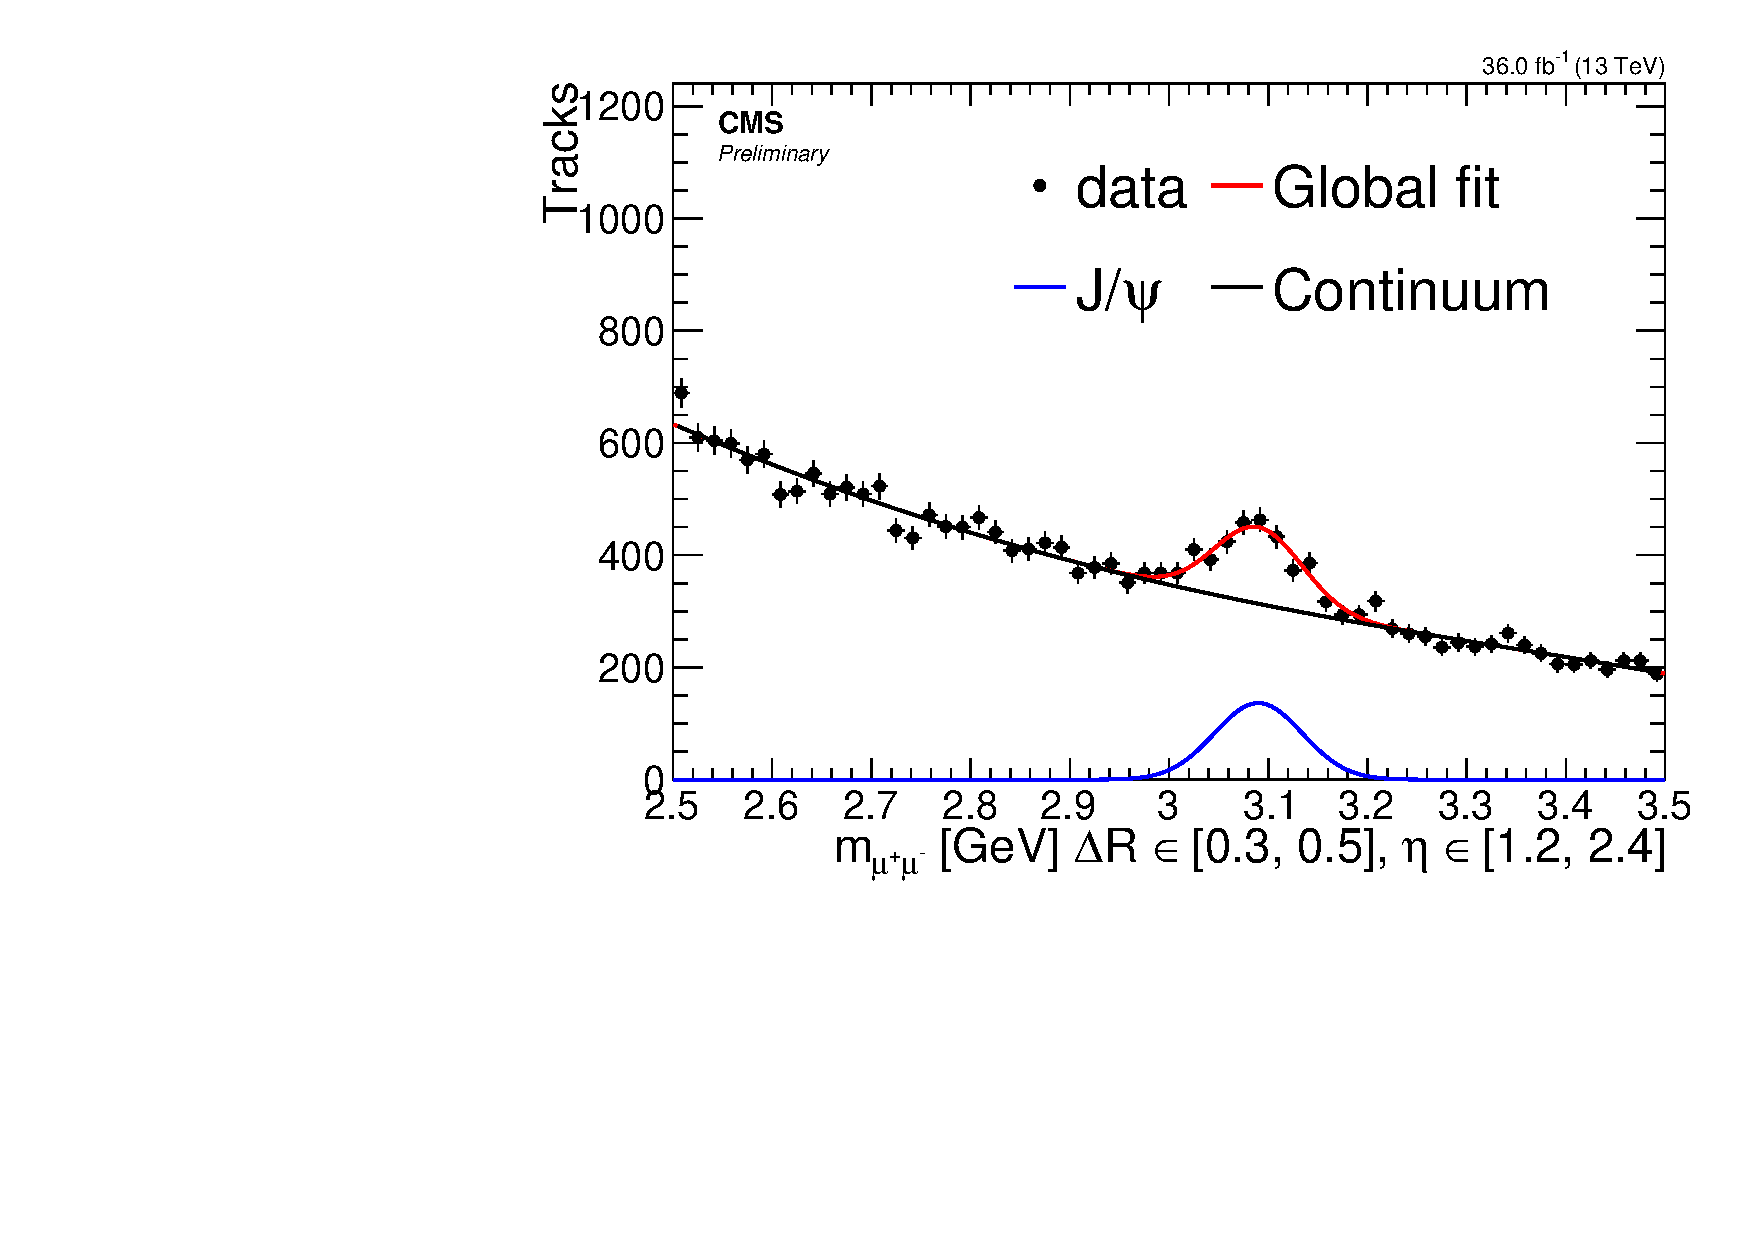
\includegraphics[width=0.32\linewidth]{plots/jpsi_muons_fit_data_delta_r_single_electron/none_invMass_0.3_0.5_1.2_2.4.pdf} \,
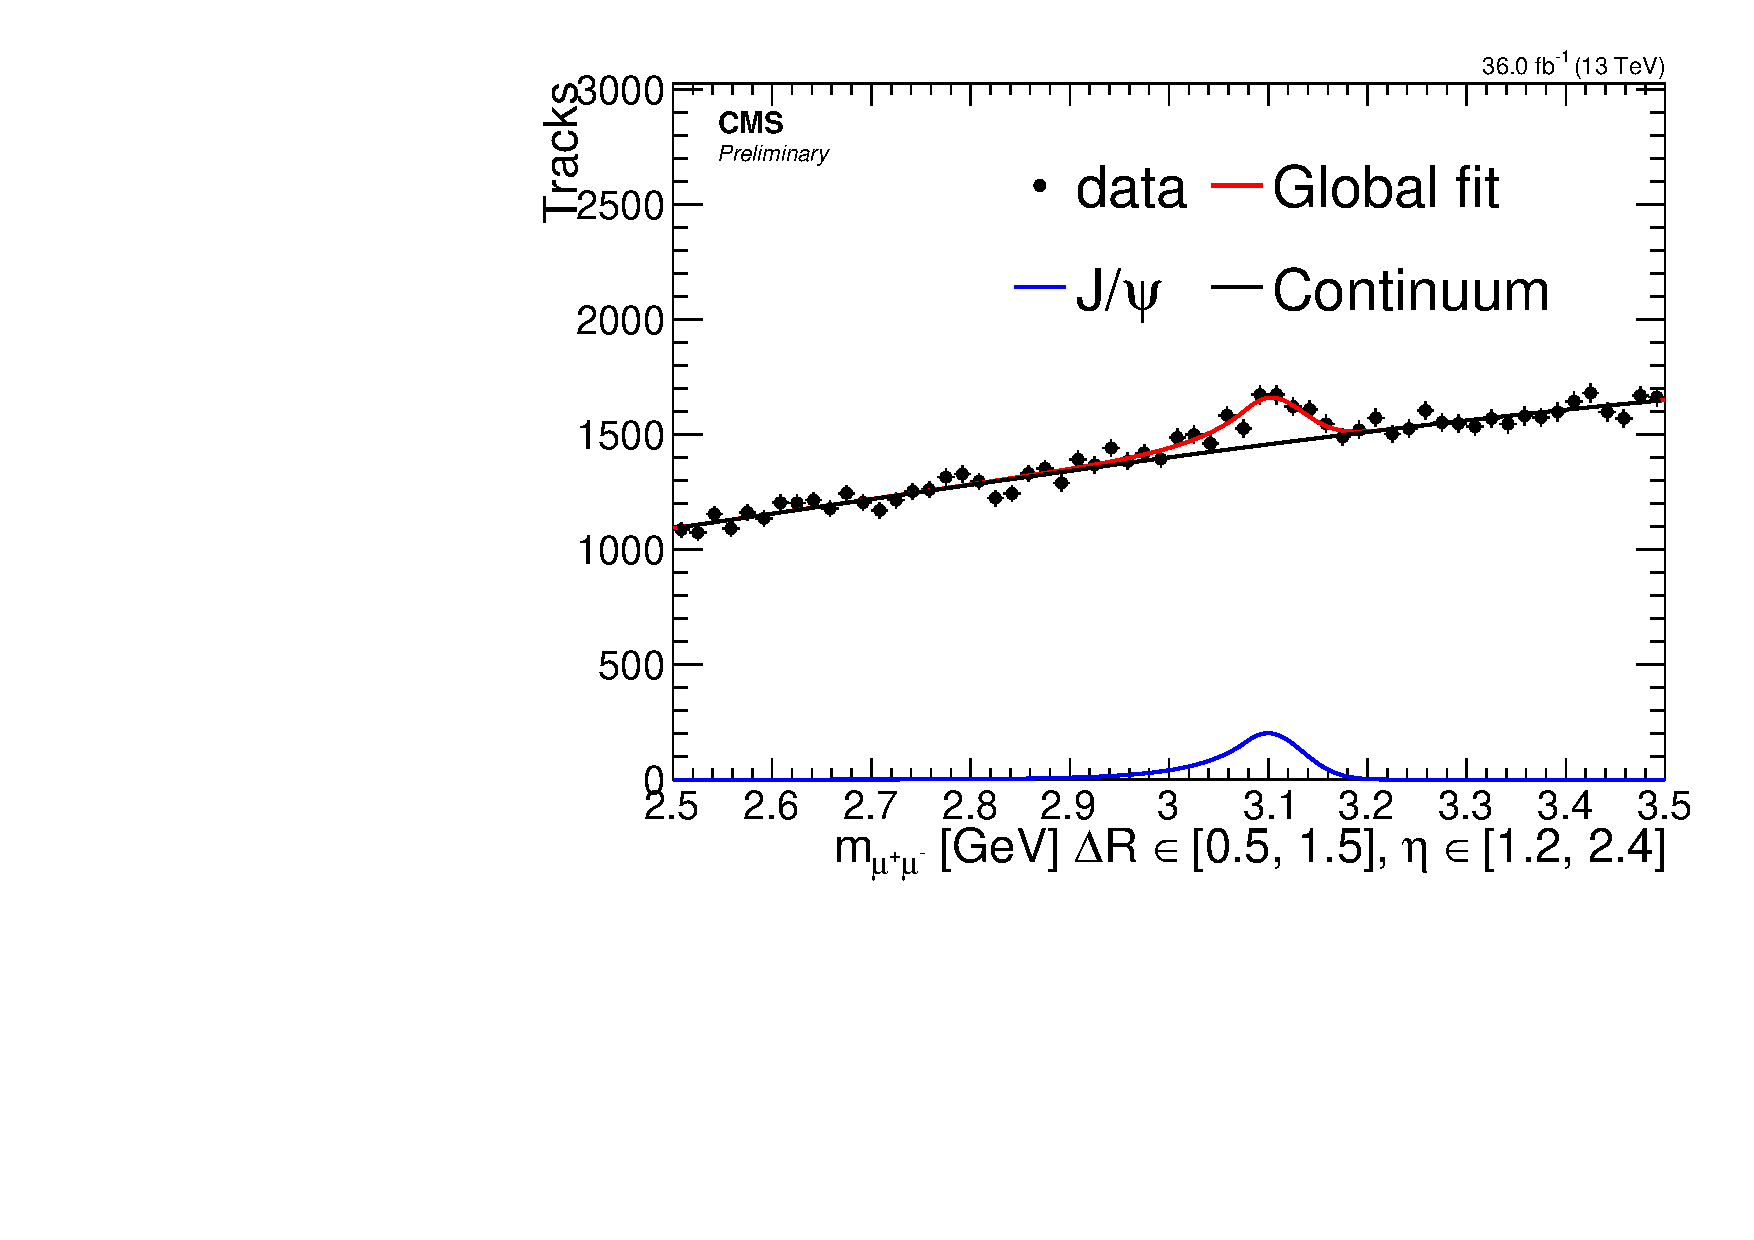
\includegraphics[width=0.32\linewidth]{plots/jpsi_muons_fit_data_delta_r_single_electron/none_invMass_0.5_1.5_1.2_2.4.pdf} \\
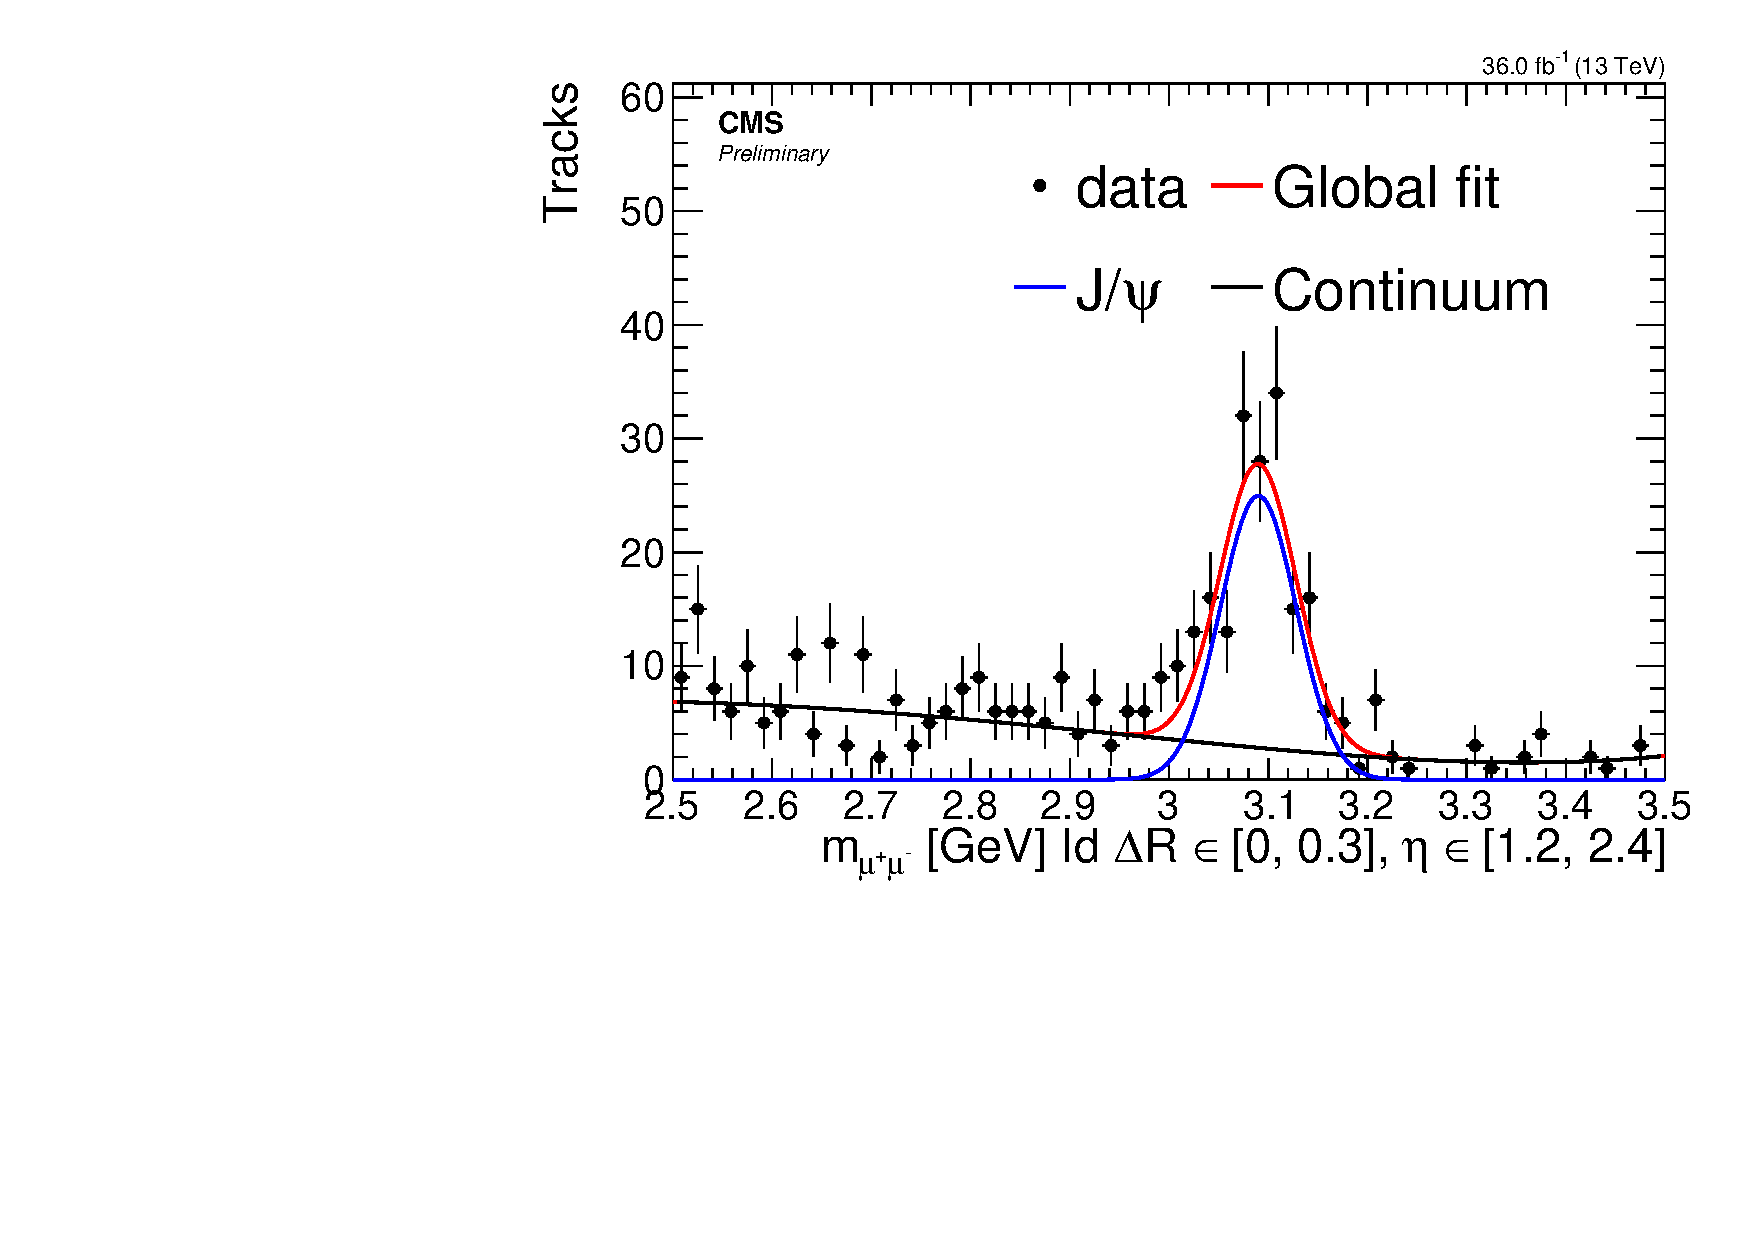
\includegraphics[width=0.32\linewidth]{plots/jpsi_muons_fit_data_delta_r_single_electron/none_id_invMass_0_0.3_1.2_2.4.pdf} \,
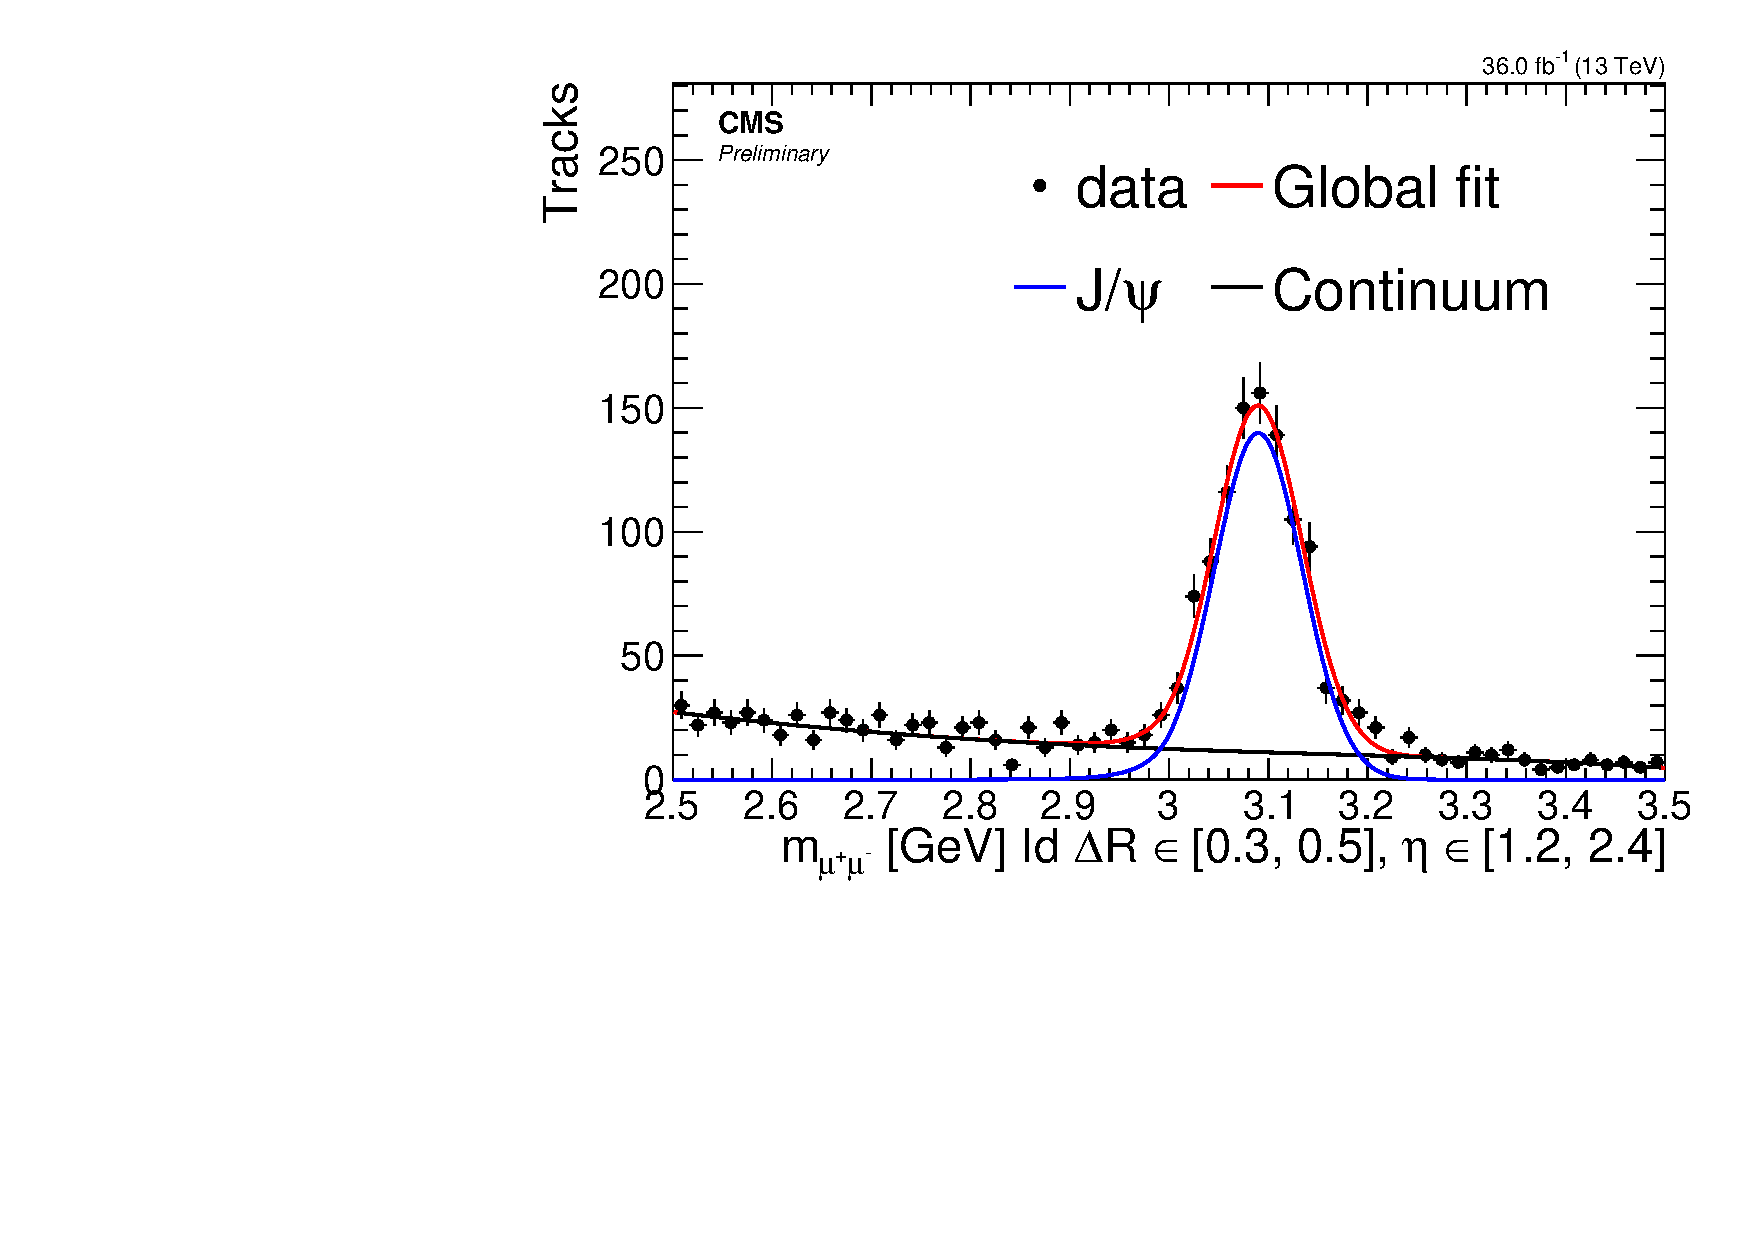
\includegraphics[width=0.32\linewidth]{plots/jpsi_muons_fit_data_delta_r_single_electron/none_id_invMass_0.3_0.5_1.2_2.4.pdf} \,
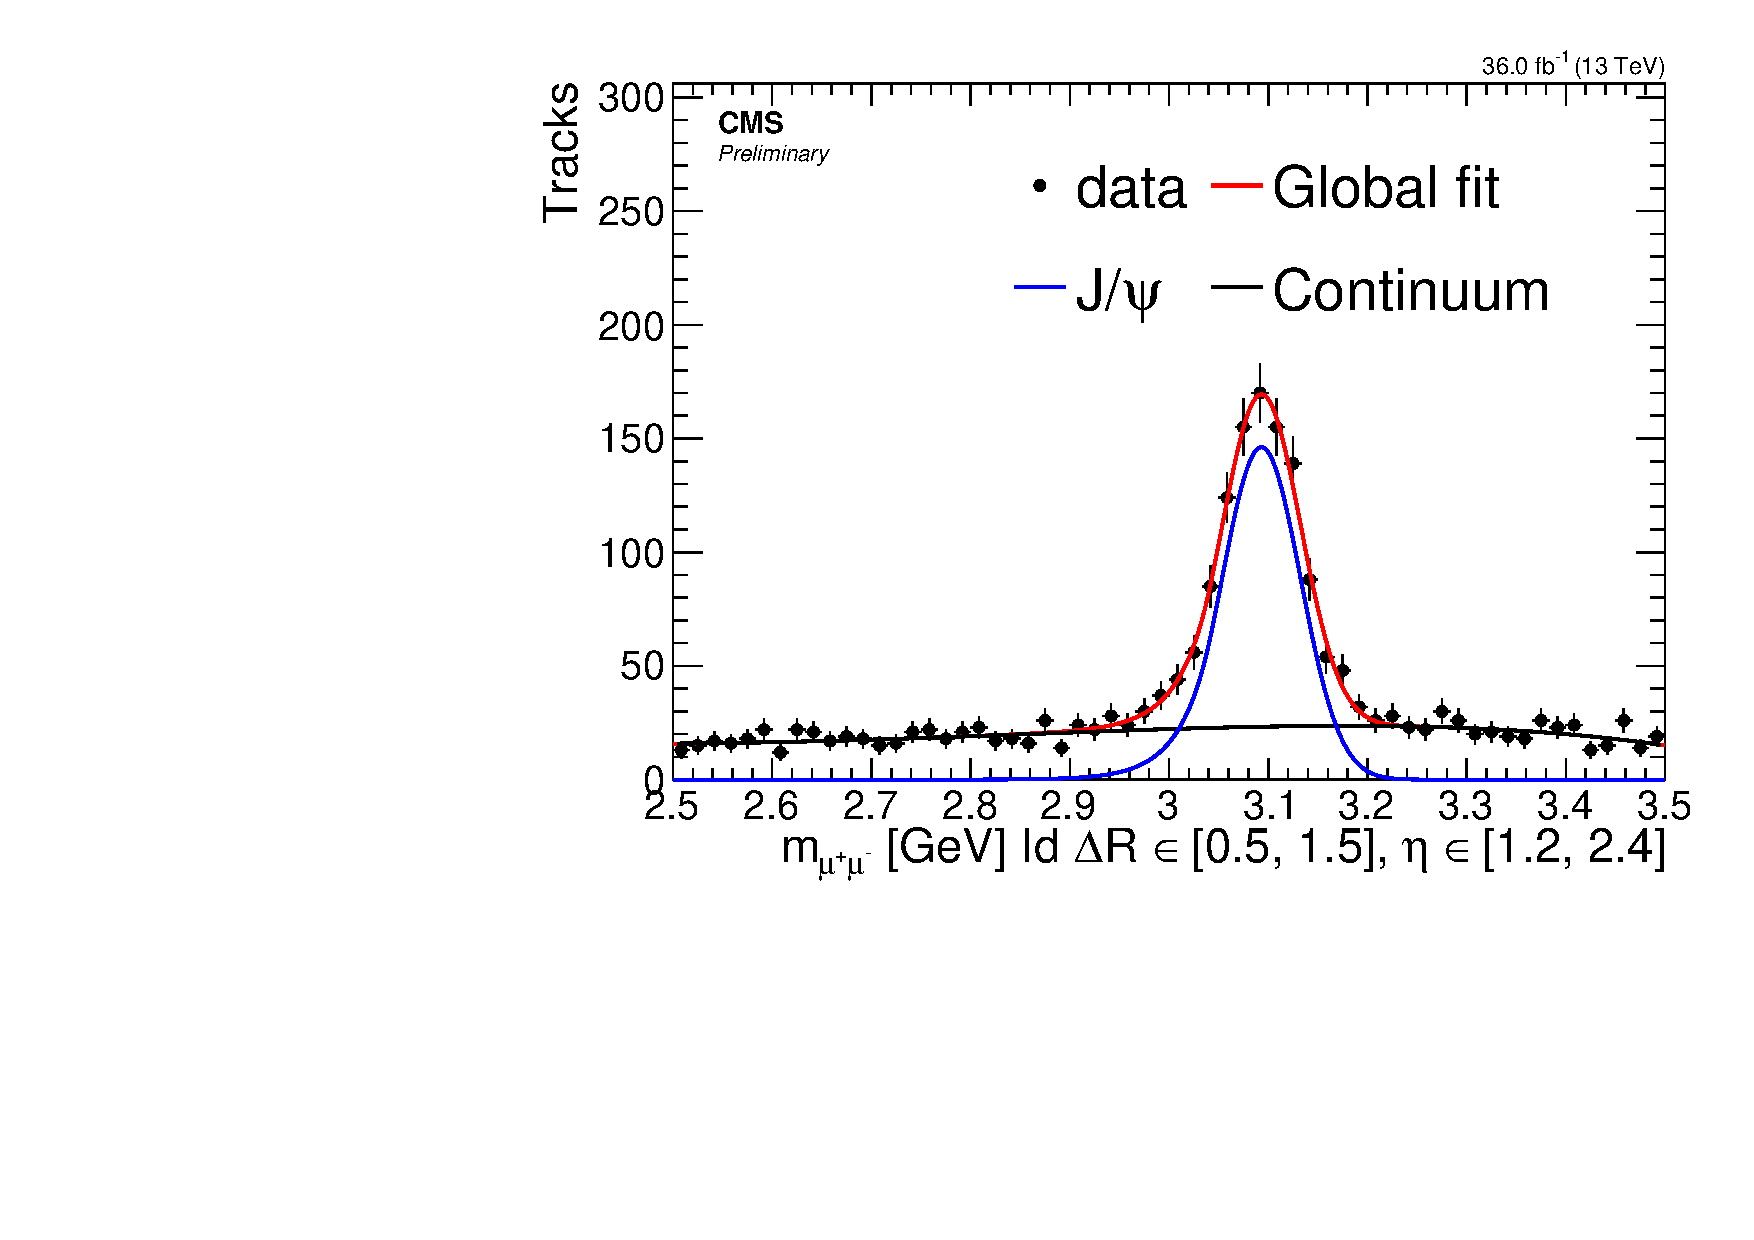
\includegraphics[width=0.32\linewidth]{plots/jpsi_muons_fit_data_delta_r_single_electron/none_id_invMass_0.5_1.5_1.2_2.4.pdf}  \\
\caption[Data endcaps muons fits]{Data endcaps muons fits for denominator (top) and numerator (bottom) for $0<\DR<0.3$  (left), $0.3<\DR<0.5$ (center), $0.5<\DR<1.5$ (right)}
\label{fig:tb-endcaps-data}
\end{figure}

The efficiencies and corresponing scale factors can be seen in ~\ref{fig:tb-eff-sf}. The scale factors are statistically consistent with unity, and show no discernible $\DR$ dependence. A similar study has been carried out with simulation and data for 2017 and 2018 in~\cite{muon-id-sf-2017-8} and did not observe a $\DR$ dependence either. The recommendation from the \gls{pog} as a results of these studies are to use the calculated scale factors provided by them with an additional systematic of 1\% for muons with $\pt<20\GeV$.

\begin{figure}[!htbp]
\centering
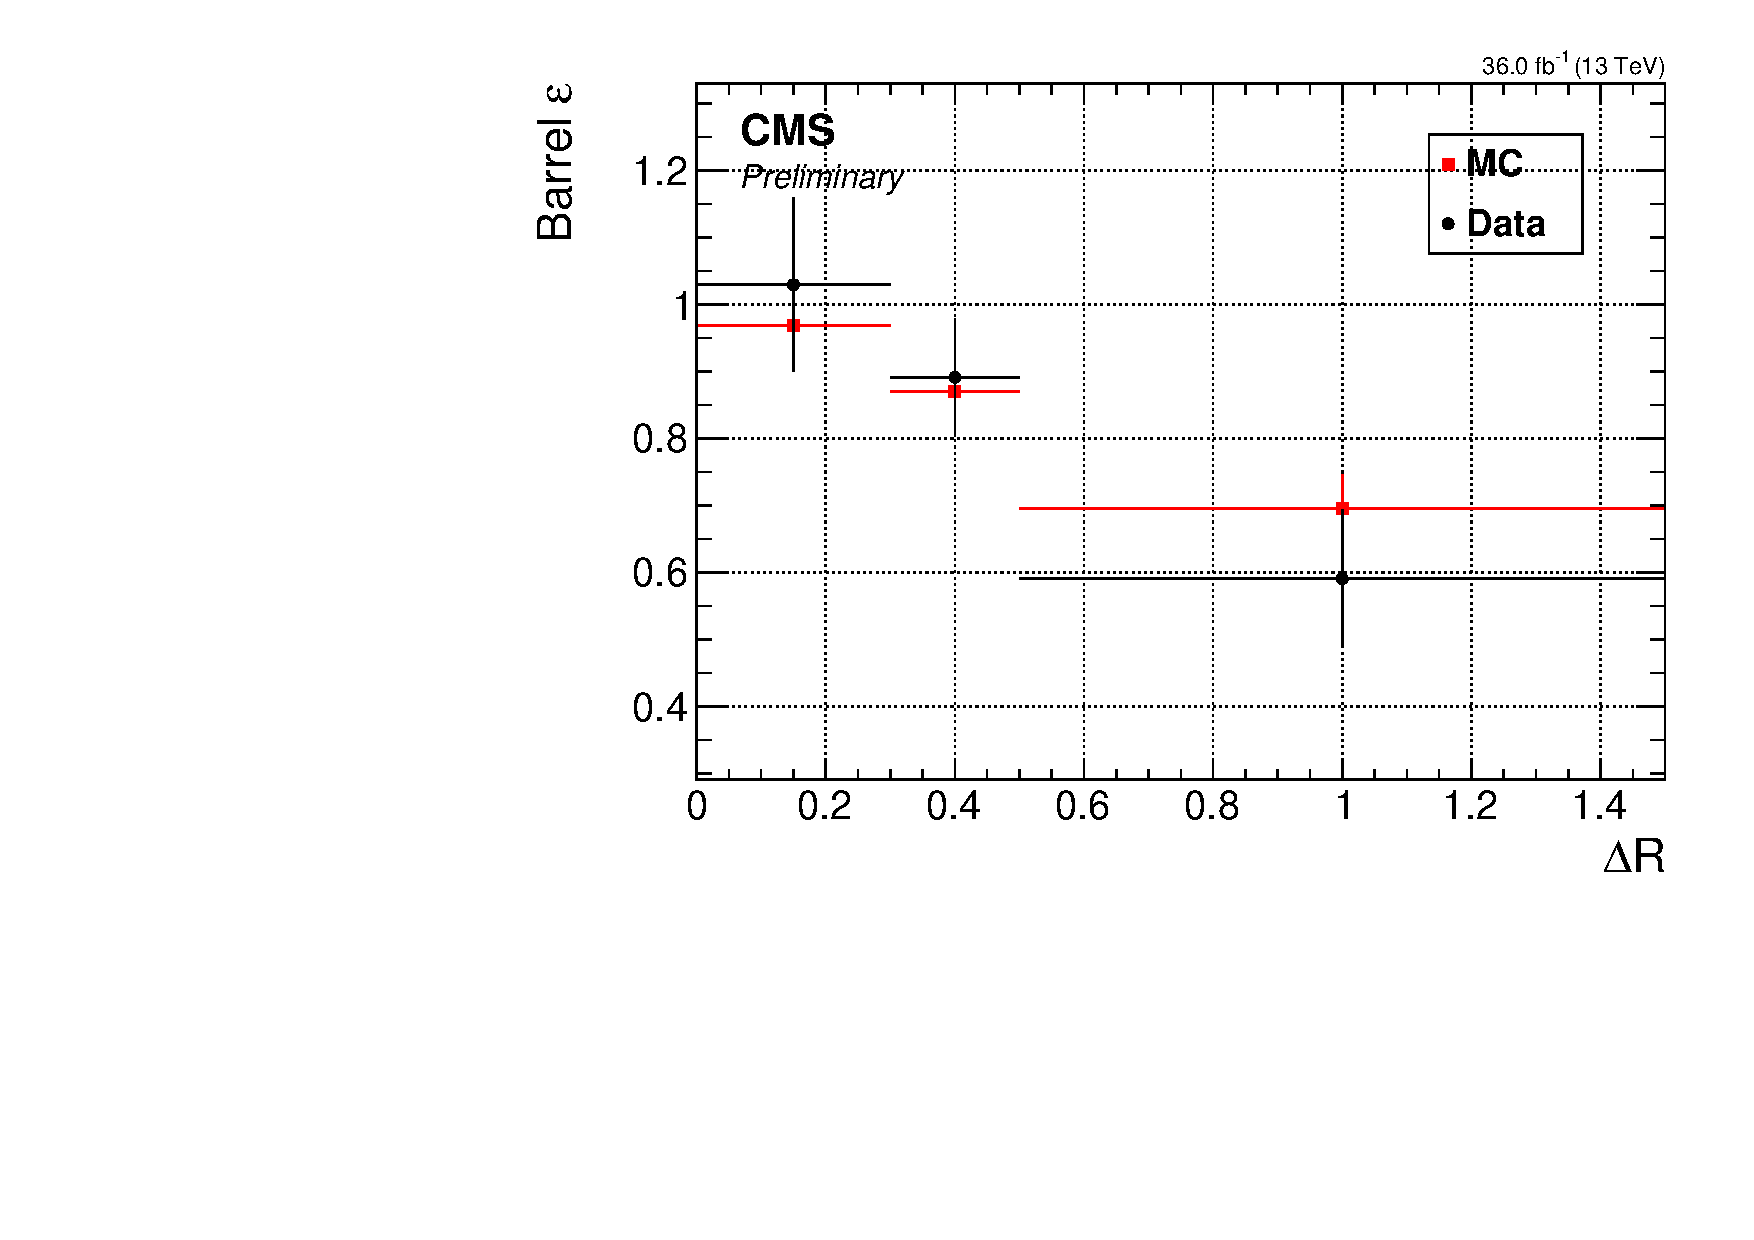
\includegraphics[width=0.48\linewidth]{plots/scale_factors/barrelDeltaRSingleElectron.pdf} \,
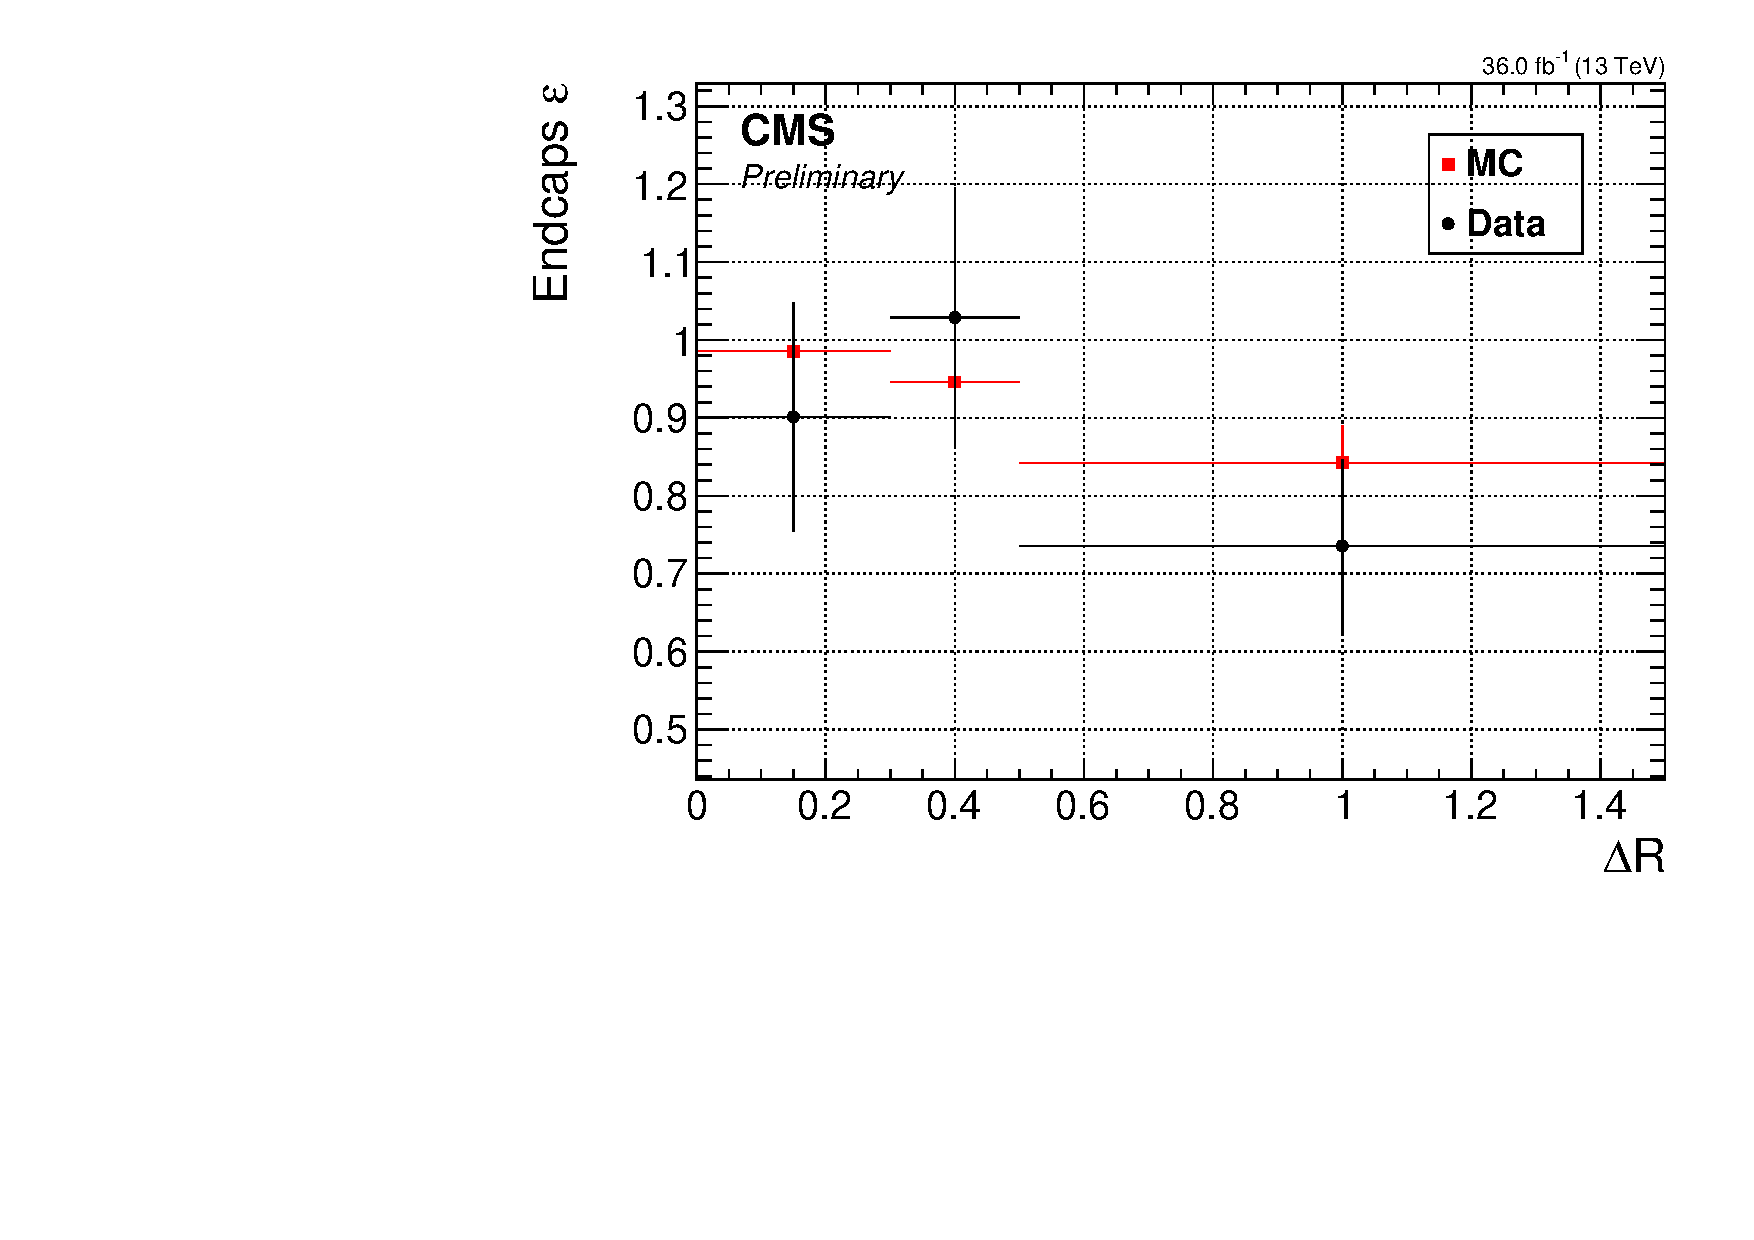
\includegraphics[width=0.48\linewidth]{plots/scale_factors/endcapsDeltaRSingleElectron.pdf}  \\
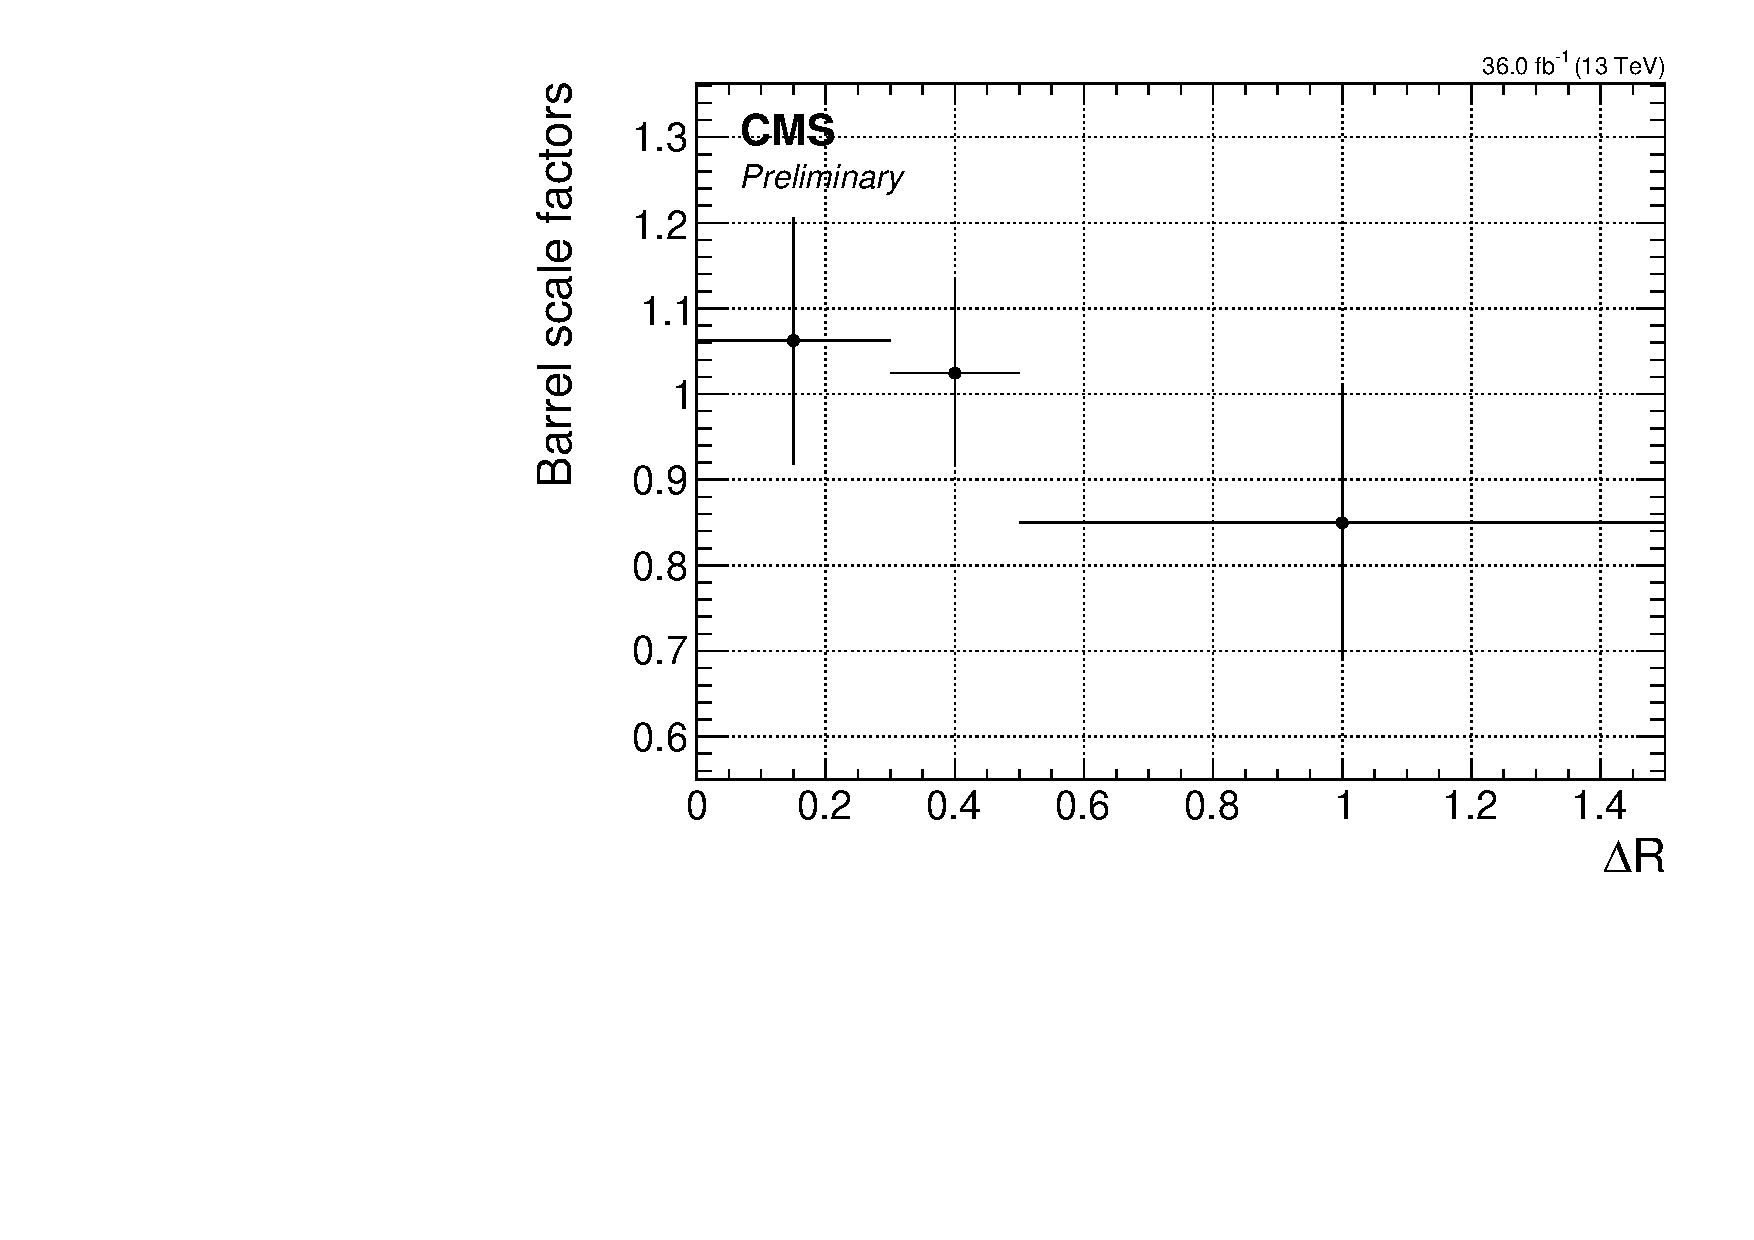
\includegraphics[width=0.48\linewidth]{plots/scale_factors/barrelDeltaRisoScaleFactorsSingleElectron.pdf} \,
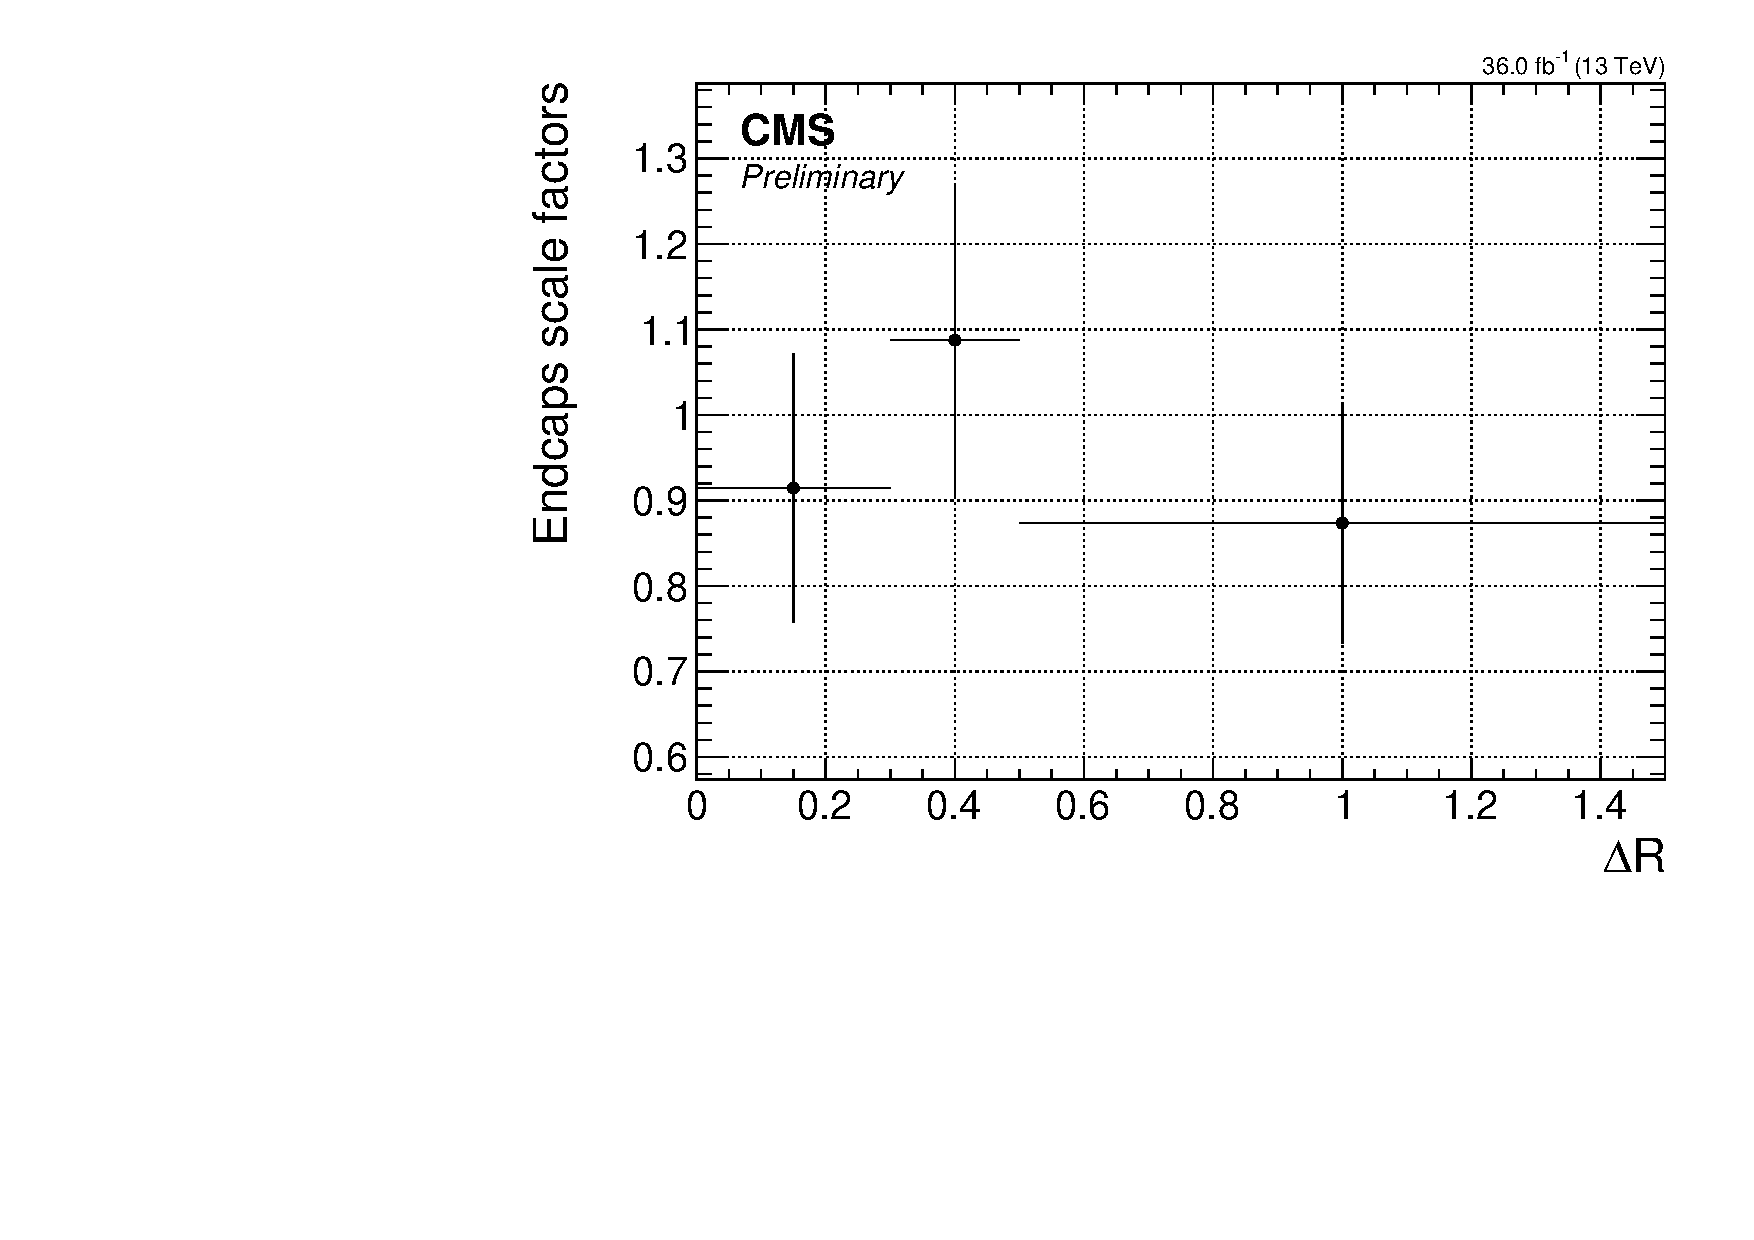
\includegraphics[width=0.48\linewidth]{plots/scale_factors/endcapsDeltaRisoScaleFactorsSingleElectron.pdf} \\
\caption[Efficiencies and scale factors]{Efficiencies (top) and scale factors (bottom) for barrel muons (left) and endcaps muons (right).}
\label{fig:tb-eff-sf}
\end{figure}